\documentclass[12pt]{article}

% Localization
\usepackage[utf8]{inputenc}
\usepackage[danish]{babel}
\usepackage[T1]{fontenc}

% Design
\usepackage{transparent}
\usepackage{fancyhdr}
\usepackage{siunitx}
\usepackage{parskip}
\usepackage{xcolor}

% Maths
\usepackage{mathtools}
\usepackage{amsfonts}
\usepackage{amssymb}
\usepackage{gensymb}
\usepackage{amsmath}
\usepackage{amsthm}
\usepackage{calc}

% Plotting
\usepackage{pgfplots}

% Bibliography
\usepackage[style=apa,backend=biber]{biblatex}
\usepackage{csquotes}
\usepackage{url}

% Figures
\usepackage{pdfpages}
\usepackage{graphicx}
\usepackage{chemfig}
\usepackage{caption}
\usepackage{float}

% Tables
\usepackage{booktabs}
\usepackage{enumitem}
\usepackage{multicol}
\usepackage{multirow}
\usepackage{array}

% Hyperref
\usepackage{hyperref}

% Definitions
\pgfplotsset{compat=1.18}
\pdfminorversion=7

\renewcommand{\subsectionmark}[1]{\markright{#1}}
\renewcommand*\printatom[1]{\ensuremath{\mathsf{#1}}}
\setlength{\headheight}{14.49998pt}
\setchemfig{scheme debug=false}

\hypersetup{linkcolor=black}

\pagestyle{fancy}
\fancyhf{}
\rfoot{\thepage}


\addbibresource{kilder.bib}
\usetikzlibrary{calc,decorations.pathmorphing,decorations.markings,patterns}

\title{KEMISK PRODUKTION \\ Syntese af parabener}
\author{Oliver Nielsen Bager, 3.A, Tradium HTX}
\date{26/4-2024} 

\begin{document}
    
    \renewcommand{\headrulewidth}{0pt}

    \pagenumbering{Roman}
    \maketitle

    \vskip 16pt

    \begin{figure}[H]\centering
        \scalebox{1.25}{
            \chemname{\chemfig{OH-*6(=-=(-C(=[7]O)(-[1]CH_{2}(-CH_{3})))-=-)}}{Ethylparaben}
        }
        \end{figure}

    \vskip 32pt
    
    \begin{figure}[H]\centering
        \scalebox{1.25}{
            \chemname{\chemfig{OH-*6(=-=(-C(=[7]O)(-[1]CH_{2}(-CH_{2}(-CH_{3}))))-=-)}}{Propylparaben}
        }
    \end{figure} 

    \thispagestyle{fancy}

    \pagebreak

    \tableofcontents

    \pagebreak

    \renewcommand{\headrulewidth}{1pt}
    \lhead{Molekylær teknologi}
    \chead{3.A}
    \rhead{Oliver Bager}
    \setcounter{page}{1}
    \pagenumbering{arabic}

    \section{Indledning}
    Konserveringen af fødevarer har gennem tiden spillet en enorm rolle for menneskets overlevelse som art. At kunnet bevare fødevarer gennem perioder med mangel, har gjort det muligt at have adgang til mad hele året rundt. 

    I nutiden, hvor forsyningen af mad ikke er et problem grundet globaliseringen, har bevaringen af mad fået en ny rolle, nemlig at muliggøre transportation og langvarig opbevaring af egnede fødevarer \parencite{Elis2019}.

    Før i tiden benyttedes oftest ``naturlige'' metoder til at konservere fødevarer, eksempler på disse kunne være: 
    \begin{itemize}
        \item[-] saltning af kød, hvilket medfører dehydrering og derved værre miljø for bakterievækst
        \item[-] tørring af frugt, grøntsager, medfører igen dehydrering
        \item[-] syltning, placerer fødevaren i et syrligt miljø hvilket minimerer bakterievækst
        \item[-] frysning, reducerer enzymaktiviteten drastisk og fryser vandet hvilket gør det ubrugeligt for mikroorganismer
        \item[-] rygning, dræber overfladebakterier og tørrer den ud, røg indeholder formaldehyd og alkohol som har bevarende virkning
    \end{itemize}
    I dag benyttes ofte i stedet syntetiske konserveringsmidler der produceres i laboratorier, grundet deres bedre effektivtet, stabilitet og omkostning. Derudover minimeres også varians mellem partier af konserveringsmidler, hvilket medfører konsekvent bevaring.

    Dæmonisering af syntetiske tilsætningsstoffer har dog medført at mange er bange for de syntetiske konserveringsmidlers indvirkning på menneskets sundhed, på trods af manglende empirisk data der understøtter dette. 

    Dette har medført at nogle producenter er begyndt at bevæge sig mod de ``naturlige''-- eller alternative konserveringsmidler med mindre data der understøtter deres inerte helbredspåvirkning for at appelere til forbrugerne, hvilket kan vise sig at have konsekvenser senere hen grundet den større eksponering til mindre velundersøgte-- og potentielt sundhedsskadelige stoffer.


    
    \section{Teori}
    \subsection{Parabener}
    Parabener indgår i en gruppe af estere dannet ved kondensationereaktion mellem 4-hydroxybenzoesyre og en vilkårlig alkohol. Afhængigt af alkoholen der benyttes vedhæftes forskellige alkylgrupper, hvilket ændrer egenskaberne af det endelige molekyle:
    \begin{figure}[H]
        \resizebox{\textwidth}{!}{
            \schemestart
            \chemname{\chemfig{OH-(*6(=-=(-COOH)-=-))}}{4-hydroxybenzoesyre}
            \+
            \chemname{\chemfig{ROH}}{Alkohol}
            \arrow(.mid east--.mid west){->[H$^+$][varme]}
            \chemname{\chemfig{OH-(*6(=-=(-COOR)-=-))}}{Paraben}
            \schemestop
        }
        \caption{Kondensationsreaktion mellem 4-hydroxybenzoesyre og vilkårlig alkohol, dannet vandmolekyle udeladt.}
    \end{figure}
    Afhængigt af hvor de skal benyttes, er det derfor også fordelagtigt at udvælge parabener med foretrækkelige egenskaber. Eksempelvis ses methylparaben oftest benyttet i levnedsmidler grundet dets højere opløselighed i vandige faser, mens blandinger-- eller parabener med længere alkylkæder oftest vil benyttes i kosmetik.
    \begin{table}[H]\centering
        \caption{Fysiske egenskaber af forskellige parabener \parencite{PubChem}.}
        \begin{tabular}{ccccc}
            \toprule
            & \multicolumn{2}{c}{Opløselighed $\left[\si{mg\per mL}\right]$} & & \\
            \cmidrule(r){2-3}
            Paraben & Vand & Ethanol & MV $\left[\si{g\per mol}\right]$ & SMP $\left[\si{\degree C}\right]$ \\
            \midrule
            Methylparaben & 2.5 & 408 & 152.15 & 125 \\
            Ethylparaben & 0.85 & 550 & 166.17 & 117 \\ 
            Propylparaben & 0.5 & 746 & 180.2 & 96 \\
            Butylparaben & 0.21 & 1649 & 194.23 & 68 \\
            \bottomrule
        \end{tabular}
    \end{table}
    Alternativt kan typisk ester--navngivning også benyttes, dog angives parabener hyppigst ved navnet på deres alkylkæde efterfulgt af \textit{paraben}, eksempelvis: \textit{ethylparaben}. \textit{Paraben} stammer fra navnet på 4-hydroxybenzoesyre. Alternativ navngivning jf. de relative molekylepositioner villet medføre at den kaldes \textit{p}-hydroxybenzoesyre, grundet hydroxygruppens placering i \textit{para}-positionen, derfra kommer \textit{para}-hydroxy\textit{ben}zoesyre.

    \subsubsection{Virkningsmekanisme}
    Parabeners virkningsmekanisme er ikke veletableret, og det er endnu ikke fuldstændigt sikkert hvordan de hindrer mikroorganismers vækst. Nogle populære teorier bygger dog på at de \parencite{Nell2001}:
    \begin{itemize}
        \item[-] forstyrrer af membrantransportprocesser
        \item[-] inhiberer DNA-- og RNA--syntese
        \item[-] inhiberer dannelsen af nødvendige enzymer som ATPase og fosfotransferase
    \end{itemize}
    Samtidigt observeres også et sammenhæng mellem længden af den vedhæftede alkylkæde og deres hæmmende effekt \parencite{Alli2005}. Dette begrundes i den faldende polaritet af molekylet i takt med at længde på alkylkæden stiger, hvilket gør det nemmere for den at interagere med den lipide cellemembran.

    Dog er dette ufordelagtigt i en række af produkter, da det begrænser muligheden for at benytte dem i varer med vandige faser. Det samme observeres også i to--fasede produkter, hvor der ofte benyttes blandinger af parabener for at sørge for at de ikke blot akkumulerer i fasen hvori de har lettest ved at forblive opløst.

    \subsubsection{Sundhedsmæssig indvirkning}
    Bekymring for den sundhedsmæssige indvirkning af en lang række syntetiske produkter bringes ofte op i medierne, samt af offentligheden generelt. Dog er dette oftest uden belæg, og kan hovedsageligt tilskrives den \textit{naturalistiske fejlslutning} --- troen på at ``naturlige'' produkter \textbf{altid} er bedre for en sundhedsmæssigt, end syntetiske alternativer, hvilket selvfølgelig ikke er sandt.

    Dette understøttes også af den eksisterende empiriske data, hvor langt størstedelen deraf viser at parabener ikke har nogen negativ indvirkning på menneskets sundhed under realistiske forhold.

    En stor del af frygten for parabener kan tilskrives tidligere studier der har påvist endokrin forstyrrelse i mus og rotter \parencite{Phil2008}, samt fund af intakte parabener i kræftramt brystvæv \parencite{Darb2004}. Senere studier har dog påvist at der ikke lader til at være et kausativt samhæng mellem eksponering for parabener og udvikling af cancer \parencite{Emil2022}, samtidigt med at den østrogeniske effekt af parabener \textit{in vivo} er dokumenteret til i værste tilfælde at være $10\cdot 10^3$ gange lavere end endogent produceret estradiol \parencite{Edwi1998}, og anses derfor for at være ubetydelig i realistiske eksponeringsmængder.

    Nogle studier har dog også vist en forhøjet endokrin forstyrrende virkning hos parabener med længere alkylkæder-- eller forgreninger \parencite{Ebru2013}, hvilket bidragede til at brugen af isopropyl-- og butylparaben blev ulovliggjort i kosmetiske produkter beregnet til børn i Danmark \parencite{Milj2013}, samt levnedsmidler i EU.
    \begin{figure}[H]\centering
        \resizebox{0.75\textwidth}{!}{
            \chemfig{OH-*6(=-=(-C(=[7]O)(-[1]O(-CH(-[1]CH_{3})(-[7]CH_{3}))))-=-)}
        }
        \caption{Isopropylparaben, en forgrenet paraben.}
    \end{figure}
    På baggrund af den manglende evidens for betydningsfulde sundhedsmæssige konsekvenser ved indtag af parabener er der dog mange der mener at de eksisterende grænseværdier \parencite{Euro2011} ikke har belæg. Samtidigt tager meget lidt af den empiriske data udgangspunkt i mennesker, og retningslinjerne er derfor udformet med udgangspunkt i dyrestudier \parencite{Emma2016}.

    Dog er brugen af methyl--, ethyl--, propyl-- og butylparaben erklæret harmløst i kosmetik indenfor en grænseværdi af EUs videnskabskomitte, mens det ikke har været muligt at drage definitive konklusioner for isopropyl--, isobutyl--, phenyl--, benzyl-- og pentylparabener grundet manglende data \parencite{Henr2013}, og brugen deraf er derfor forbudt. En acceptabel daglig dosis for summen af methyl-- og ehtylparaben fra levnedsmidler er $0-10\si{mg\per kg}$

    Disse værdier er i praksis nærmest umulig at overskride. Et spansk studie \parencite{Yola2020} fandt et gennemsnitligt parabenindhold på $73.86\si{ng\per g}$, ved undersøgelse af 98 forskellige levnedsmidler fra et supermarked, hvilket medfører at en gennemsnitlig person ($m=70\si{kg}$) skulle indtage ca.\ $9.5\si{t}$ levnedsmidler for at nå grænseværdien.
    
    Med udgangspunkt i den eksisterende litteratur er det derfor svært at opstille et kausativt sammenhæng mellem brugen af parabener og en negativ sundhedsmæssig indvirkning. På trods af konstant granskning siden deres første dokumenterede brug i 1920'erne \parencite{Mary1984}, eksisterer stadig ikke bevis for parabeners negative sundhedspåvirkning, hvilket videre bidrager til argumentationen for deres brug i både kosmetik samt levnedsmidler. 

    Flere undersøgelser, specielt i mennesker, er dog nødvendige for at opstille en definitiv konklusion for indtagsgrænserne, og de er derfor sat relativt konservativt. Dog er de kategoriserede som GRAS (\textit{Generally Recognized as Safe}) af Amerikas levnedsmiddelsstyrrelse \parencite{FDA2022}.

    \subsubsection{Nedbrydning}
    \textit{In vivo} nedbrydes parabener hovedsageligt i leveren eller huden afhængigt af hvordan de er optagede (dermal applikation vs.\ levnedsmiddel) ved 2--faset metabolisering. I den første fase hydrolyseres molekylet ved enzymatisk reaktion med en carboxylesterase--isoform (CES-1 i leveren, CES-2 i huden) afhængigt af optagelsessitet, hvilket resulterer i omdannelsen til 4-hydroxybenzoesyre og den korresponderende alkohol der herefter udskilles gennem urinen.
    \begin{figure}[H]
        \resizebox{\linewidth}{!}{
            \schemestart
            \chemfig{OH-*6(=-=(-COOR)-=-)}
            \+
            \chemfig{H_{2}O}
            \arrow{->[CES]}
            \chemfig{OH-*6(=-=(-COOH)-=-)}
            \+
            \chemfig{R-OH}
            \schemestop
        }
        \caption{Endogen hydrolysering af paraben ved enzymatisk reaktion med carboxylesterase.}
    \end{figure}
    Den 2.\ fase af metaboliseringen sker ved glukoronidation af de tilbageværende relativt upolære molekyler, katalyseret af glukoronosyltransferase--enzymet (UGT), hvilket medfører en polaritetsstigning hvorved de kan elimineres gennem urinen.
    \begin{figure}[H]
        \resizebox{\linewidth}{!}{
            \schemestart
            \chemfig{*6(=(-[6]OH)-=-(-COOR)=-)}
            \+
            \chemfig{HO-R}
            \arrow(.mid east--.mid west){->[UGT]}
            \chemfig{O(-[4]*6(-(-CH(=[2]O))-O-(-OH)-(-OH)-(-OH)-))(-[1]C(=[2]O)(-[7]*6(=-=-=-=(-OH)-)))}
            \+
            \chemfig{*6((-OH)-(-OH)-(-OR)-(-CH(=[7]O))-O-(-OH)-)}
            \schemestop
        }
        \caption{Glukoronidation af tilbageværende relative upolære molekyler, 2 vandmolekyler udeladt.}
    \end{figure}
    I plasma lader det til at parabener med kortere alkylgrupper er stabile, mens parabener med længere alkylgrupper degraderes over tid. Den effektive nedbrydning af parabener i leveren indikerer at de \textit{ikke} akkumulerer i kroppen over tid, og i stedet elimineres fuldstændigt \parencite{Suza2010}.

    For kosmetiske produkter indeholdende parabener hydrolyseres de igen ved enzymatisk reaktion med carboxylesterase, dog denne gang ved isoform 2, CES2, hvilket igen medfører at en meget lille mængde af parabenen når at komme i cirkulation, hvorefter de igen elimineres i leveren.

    Samtidigt observeres det at parabener med længere alkylkæder generelt hydrolyseret hurtigere i huden, mens parabener med kortere alkylkæder hydrolyseres hurtigere i leveren. Dette er grundet forskellene på de 2 isoformer af carboxylesterase, hvor CES1 har en præference for korte alkylkæder og store acylgrupper, mens at CES2 har det omvendte \parencite{Cath2021}.

    \subsection{Synteseprocessen}
    Parabener dannes ved syre--katalyseret esterificering af 4-hydroxybenzoesyre og en vilkårlig alkohol. Dette sker ved at protonen i carboxylsyregruppen fraspaltes under kondensationsreaktion med alkoholens hydroxygruppe, hvorved dets alkylkæde vedhæftes ved oxygenmolekylet ved fraspaltning af et vandmolekyle.

    Som katalysator i denne proces benyttes koncentreret svovlsyre. Under en Fischer--esterificeringsreaktioner benyttes stærke organiske syrere for at muliggøre dannelsen af en carbokat--ion, hvilket muliggør nukleofil addition \parencite{Stev2023}. Dette gøres ved at den stærke syre overfører en proton til det carbonyle oxygenatom hvilket er muligt grundet elektronegativitetsforskellen. Dette medfører en stigning i det carbonyle carbon--atoms elektrofilicitet ved dannelse af en carbokat--ion.
    \begin{figure}[H]
        \resizebox{\linewidth}{!}{
            \schemestart
            \chemfig{C(-[::-30]OH)(=[2]@{DB2}\charge{45=\:,135=\:}{O})(-[::-150]R)}
            \+
            \chemfig{@{DB1}H^{+}}
            \arrow{->}
            \chemfig{C(=[@{DB3}2]@{DB4}O^{+}(-[::-60]H))(-[::-30]OH)(-[::-150]R)}
            \arrow{->}
            \chemfig{C^{+}(-[::-30]OH)(-[::-150]R)(-[2]OH)}
            \schemestop
            \chemmove{
                \draw[-stealth] ($(DB1)+(0,0.2)$) to[bend right=100,looseness=1.1] ($(DB2)+(0,0.3)$);
                \draw[-stealth] ($(DB3)+(0.125,0)$) to[bend right=65,looseness=2] ($(DB4)+(0.2,-0.1)$);
            }
        }
        \caption{Dannelse af carbokat--ion under reaktion med stærk syre.}
    \end{figure}
    Alkoholen har i denne reaktion mulighed for at agere som et nukleofil grundet de frie elektronpar på oxygen--atomet. En nukleofil addition sker derfor ved carbokat--ionen, hvorved alkoholen vedhæftes ved carbokat--ionen dannet, hvilket danner en oxonium--ion ved protonoverførsel.
    \begin{figure}[H]
        \resizebox{\linewidth}{!}{
            \schemestart
            \chemfig{@{DB2}C^{+}(-[::-30]OH)(-[::-150]R)(-[2]OH)}
            \+
            \chemfig[baseline=10pt]{@{DB1}\charge{-45=\:,-135=\:}{O}(-[::30]H)(-[::150]R)}
            \arrow(.mid east--.mid west){->}
            \chemfig[baseline=-5pt]{C(-[6]O^{+}(-[::-60]R)(-[::60]H))(-[4]R)(-O(-[::45]H))(-[2]OH)}
            \schemestop
            \chemmove{
                \draw[-stealth] ($(DB1)+(0,-0.25)$) to[bend left=75,looseness=1.3] ($(DB2)+(0,-0.25)$);
            }
        }
        \caption{Nukleofil addition af alkoholmolekyle.}
    \end{figure}
    Den dannede ether er en dårlig leaving group, og protonen overføres derfor til den ene af hydroxygrupperne hvilket medfører dannelsen af et aktiveret kompleks hvorved vandmolekylet fraspaltes. 
    \begin{figure}[H]
        \resizebox{\linewidth}{!}{
            \schemestart
            \chemfig{C(-[6]O^{+}(-[::-60]R)(-[::60]@{DB1}H))(-[4]R)(-@{DB2}\charge{-45=\:,-135=\:}{O}(-[1]H))(-[@{DB6}2]@{DB5}\charge{120=\:,210=\:}{O}(-[::-60]H))}
            \arrow{->}
            \chemfig{C(-[6]O(-[::-60]R))(-[@{DB3}]@{DB4}O^{+}(-[1]H)(-[7]H))(=[2]\charge{150=\:}{O}(-[::-60]H))(-[4]R)}
            \arrow{->}
            \chemfig{C(-[::-30]O(-[::60]R))(=[2]\charge{150=\:}{O^{+}}(-[::-60]H))(-[::210]R)}\hspace{8pt}
            \arrow{0}[,-0.125]\+
            \chemfig{H_{2}O}
            \schemestop
            \chemmove{
                \draw[-stealth] ($(DB1)+(0.2,0)$) to[bend right=65,looseness=1.25] ($(DB2)+(0.25,-0.3)$);
                \draw[-stealth] ($(DB3)+(0,0.1)$) to[bend left=75, looseness=1.5] ($(DB4)+(0,0.2)$);
                \draw[-stealth] ($(DB5)+(-0.25,-0.15)$) to[bend right=75,looseness=2] ($(DB6)+(-0.1,0)$);
            }
        }
        \caption{Dannelse af aktivt kompleks ved protonoverførsel til hydroxygruppe samt fraspaltning af vandmolekyle.}
    \end{figure}
    Hvorved det kovalente bånd mellem oxonium--ionen og hydrogen--atomet opløses, hvilket frigiver elektronen som optages af oxonium--ionen grundet elektronegativitetsforskellen, og neutraliserer ladningen.
    \begin{figure}[H]
        \resizebox{\linewidth}{!}{
            \schemestart
            \chemfig{C(-[::-30]O(-[::60]R))(=[2]@{DB2}\charge{150=\:}{O^{+}}(-[@{DB1}::-60]H))(-[::210]R)}
            \arrow{->}
            \chemfig{C(-[::-30]O(-[::60]R))(-[::210]R)(=[2]\charge{45=\:,135=\:}{O})}\hspace{10pt}
            \arrow{0}[,-0.1]\+
            \chemfig{H^{+}}
            \schemestop
            \chemmove{
                \draw[-stealth] ($(DB1)+(0,-0.1)$) to[bend left=75,looseness=1.5] ($(DB2)+(0.2,-0.1)$);
            }
        }
        \caption{Neutralisering af ladning ved frigivelse af hydron.}
    \end{figure}
    Da hydronerne ikke opbruges under reaktionen er det nødvendigt at neutralisere opløsningen for at gøre den sikker at håndtere. Dog er det også nødvendigt at genkende at dette er en ligevægtsreaktion: 
    \[
    \mathrm{C_7H_6O_3+ROH} \rightleftarrows \mathrm{C_7H_5O_3R+H_2O}
    \] 
    Hvilket medfører at det vil være optimalt at udføre et indgreb der forskyder ligevægten mod produktsiden. Ideelt villet vi kunnet fradestillere vandet under reaktionen, men grundet dets højere kogepunkt end de benyttede alkoholer er dette ikke en mulighed. Vi tilsætter derfor alkohol i overskud.
    
    \subsection{Smeltepunktsbestemmelse}
    Smeltepunktsbestemmelse gør det muligt at få en generel ide om et molekyles struktur. Et givent molekyles smeltepunkt er hovedsageligt bestemt af hvor tæt molekylet kan pakkes. I forbindelse med parabener vil vi derfor forvente et fald i smeltepunkt i takt med at længden af alkylkæden stiger, da der er begrænset mulighed for at danne Londonbindinger siden den aromatiske ring optager en stor volumen i rummet.

    \subsection{Tyndtlagschromatografi}
    Tyndtlagschromatografi benyttes til at analysere renheden af-- og identificere eventuelle urenheder i et givent produkt. Metoden benytter den sandsynlige polaritetsforskel af dannede molekyler til at skille dem ad. Dette gøres ved at placere stoffet på en stærkt polær plade (oftest en plade coatet med silicagel grundet dets overfladiske hydroxygrupper). 
    \begin{figure}[H]
        \resizebox{\linewidth}{!}{
            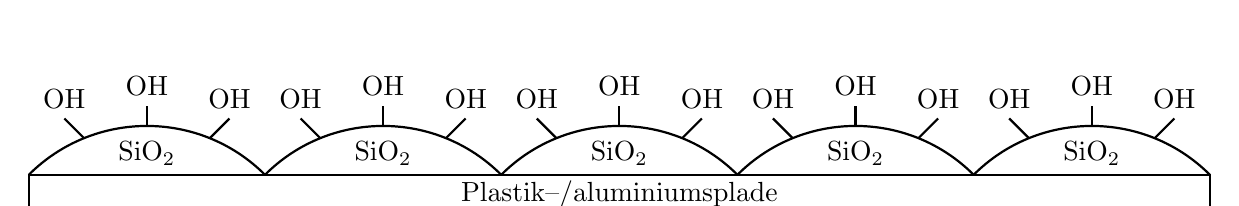
\begin{tikzpicture}
                \draw[thick] (0,0) rectangle (15,-.5);
                \node at (7.5,-.25){Plastik--/aluminiumsplade};
                \foreach \x in {0,3,6,9,12}{
                    \draw[-,thick] (\x,0) to[bend left=45] node(a)[pos=.25]{} node(b)[pos=.5]{} node(c)[pos=.75]{} ($(\x,0)+(3,0)$);
                    \draw[-,thick] ($(a)$) -- ($(a)+(-.25,.25)$) node[anchor=south]{OH};
                    \draw[-,thick] ($(b)$) -- ($(b)+(0,.25)$) node[anchor=south]{OH};
                    \draw[-,thick] ($(c)$) -- ($(c)+(.25,.25)$) node[anchor=south]{OH};
                    \node at ($(b)+(0,-.35)$){SiO$_2$}; 
            }
            \end{tikzpicture}
        }
        \caption{Illustration af hydroxygrupper på silicagel--pålagt TLC--plade.}
    \end{figure}
    Ved at tilføje en løbevæske og lade den vandre op ad pladen, vil stofferne ``trækkes'' forskellige afstande da pladen vil holde bedre fast i de polære-- end upolære stoffer.

    Endvidere giver dette også mulighed for at samligne med kommercielt indkøbte stoffer, hvor man er sikker på renhed, idet man-- hvis det korrekte produkt er dannet, ville forvente at have ens løbelængder.
    
    \subsection{Spektroskopi}
    Spektroskopi er den videnskabelige disciplin der beskæftiger sig med måling-- og studiet af frekvensspektra. Et frekvensspektra dannes ved at undersøge hvordan elektromagnetiske bølger (radiobølger, mikrobølger, infrarøde bølger, osv.) interagerer med eksempelvis molekyer \parencite{Sigu2024}. Afhængigt af deres bølgelænde tildeles de forskellige navne: 
    \begin{figure}[H]
        \resizebox{\textwidth}{!}{
            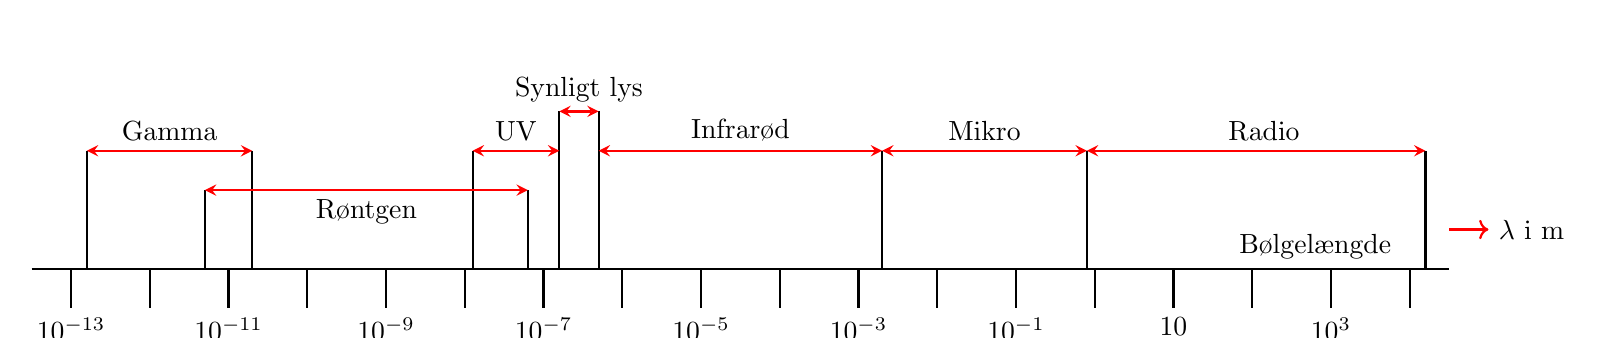
\begin{tikzpicture}
                \draw[thick] (0.5,0) -- (18.5,0);
                \foreach \x in {1,...,18}{
                    \draw[thick] (\x,0) -- (\x,-0.5);
                }
                \draw (1,-0.5) node [black,below] {$10^{-13}$};
                \draw (3,-0.5) node [black,below] {$10^{-11}$};
                \draw (5,-0.5) node [black,below] {$10^{-9}$};
                \draw (7,-0.5) node [black,below] {$10^{-7}$};
                \draw (9,-0.5) node [black,below] {$10^{-5}$};
                \draw (11,-0.5) node [black,below] {$10^{-3}$};
                \draw (13,-0.5) node [black,below] {$10^{-1}$};
                \draw (15,-0.5) node [black,below] {$10$};
                \draw (17,-0.5) node [black,below] {$10^{3}$};
                \draw[red,thick,->] (18.5,0.5) -- (19,0.5);
                \draw[thick] (19,0.5) node [black,right] {$\lambda$ i m};
                \draw[thick] (1.2,0) -- (1.2,1.5);
                \draw[thick] (3.3,0) -- (3.3,1.5);
                \draw[thick] (2.7,0) -- (2.7,1);
                \draw[thick] (6.8,0) -- (6.8,1);
                \draw[thick] (6.1,0) -- (6.1,1.5);
                \draw[thick] (7.2,0) -- (7.2,2);
                \draw[thick] (7.7,0) -- (7.7,2);
                \draw[thick] (11.3,0) -- (11.3,1.5);
                \draw[thick] (13.9,0) -- (13.9,1.5);
                \draw[thick] (18.2,0) -- (18.2,1.5);
                \draw[thick,stealth-stealth,red] (1.2,1.5) -- (3.3,1.5);
                \draw (2.25,1.5) node [black,above] {Gamma};
                \draw[thick,stealth-stealth,red] (2.7,1) -- (6.8,1);
                \draw (4.75,1) node [black,below] {Røntgen};
                \draw[thick,stealth-stealth,red] (6.1,1.5) -- (7.2,1.5);
                \draw (6.65,1.5) node [black,above] {UV};
                \draw[thick,stealth-stealth,red] (7.2,2) -- (7.7,2);
                \draw (7.45,2) node [black,above] {Synligt lys};
                \draw[thick,stealth-stealth,red] (7.7,1.5) -- (11.3,1.5);
                \draw (9.5,1.5) node [black,above] {Infrarød};
                \draw[thick,stealth-stealth,red] (13.9,1.5) -- (18.2,1.5);
                \draw (16.15,1.5) node [black,above] {Radio};
                \draw[thick,stealth-stealth,red] (11.3,1.5) -- (13.9,1.5);
                \draw (12.6,1.5) node [black,above] {Mikro};
                \draw (16.8,0) node [black,above] {Bølgelængde};
            \end{tikzpicture}
        }
        \caption{Det elektromagnetiske spektrum \parencite{Birg2012}.}
    \end{figure}
    \begin{table}[H]\centering
        \caption{Molekylær effekt og fysiske egenskaber af forskellige bølgetyper.}
        \begin{tabular}{cccc}
            \toprule
            Bølgetype & Bølgelængde $\left[\si{cm}\right]$ & Energi $\left[\si{kcal\per mol}\right]$ & Molekylær effekt \\
            \midrule
            Gamma & $10^{-9}$ & $10^6$ & \multirow{3}{*}{Ionisering} \\
            X--ray & $10^{-7}$ & $10^4$ \\
            Vakuum UV & $10^{-5}$ & $10^{-9}$ \\
            \midrule
            Tæt UV & $10^{-4}$ & $10^2$ & \multirow{2}{*}{Elektrontransistion} \\
            Synlig & $10^{-3}$ & $10$ \\
            \midrule
            Infrarød & $10^{-1}$ & $10^{-2}$ & Vibration \\
            Mikro & $10^2$ & $10^{-4}$ & Rotation \\
            Radio & $10^4$ & $10^{-6}$ & Spintransistion \\
            \bottomrule
        \end{tabular}
    \end{table}
    Når en elektromagnetisk bølge pålægges et molekyle er der en række forskellige muligheder, hvorved der konsekvent er mulighed for dannelsen af forskellige spektra der viser det enkelte molekyles spektrofotometriske egenskaber \parencite{Finn2020}:
    \begin{itemize}
        \item[1)] \textit{Absorbtionsspektrum}, kontinuert spektrum der måler et molekyles evne til at absorbere lys af en given bølgelængde (og derved energi), gør det muligt at identificere bølgelængderne som et molekyle har mulighed for at optage.
        \item[2)] \textit{Emissionsspektrum}, det modsatte af et absorbtionsspektrum, måler bølgelængderne (og derved igen energien) af den elektromagnetisk stråling der emitteres fra molekylet ved at gå fra et højt energistadie, til et lavt energistadie.
    \end{itemize}
    Det har vist sig senere hen at lys i virkeligheden ikke opfører sig som udelukkende som en bølge, men i stedet både som en partikel og bølge, kendt som bølge-partikel-dualiteten. Energien af lys er derfor ikke kontinuært, men i stedet følger det kvantemekaniske regler. Dvs.\ at energien kommer i diskrete klumper, kaldet energikvanter (fotoner). Energien af disse kan bestemmes ved Einstein-Planck relationen givet ved:
    \[
    E=hf
    \]
    Hvor $h$ er Plancks konstant, og $f$ er frekvensen af lyset \parencite{Giov2022}. Dette betyder samtidigt også at energistadierne i et molekyler må være kvantificerede, og derved diskrete \parencite{Erla2002}, hvilket medfører at hvert molekyle har deres egne absorbtionsspektra grundet forskelle i deres struktur, da et molekyle udelukkende kan absorbere fotoner med en energi der svarer til energidifferensen mellem to kvantemekaniske energistadier. Denne egenskab gør det oplagt til kemisk analyse, da det gør det muligt at differentiere mellem forskellige molekyler. Til dette formål benyttes specielt \textit{kernemagnetisk resonans spektroskopi} (NMR, samt dets undertyper som H-NMR og C-NMR) og \textit{infrarød spektroskopi} (IR), der har hver deres fordele og ulemper. 

    \subsubsection{H-NMR-spektroskopi}
    H-NMR-spektroskopi undersøger overgangen mellem kvantemekaniske energistadier, der sker når et molekyle i et ydre magnetfelt udsættes for en elektromagnetisk frekvens af den rette bølgelængde. Ved at detektere et sådant spring mellem energistadierne kan et NMR-spektrum dannes, hvilket gør det muligt at undersøge strukturen af molekyler.

    Den unikke interaktion mellem molekyler og ydre magnetfelter begrundes i deres \textit{spin}, der minder meget om vinkelmomentet vi kender fra den makroskopiske verden. Hvor spin kommer fra er enormt komplekst, og endnu ikke definitivt beskrevet gennem fysikken \parencite{Edwi2015}, det vides dog at spinnet for elektroner, protoner og neutroner er givet ved $I=\frac{1}{2}$.

    For et givent system bestående af $n$ dele der hver har et spin kan dets totale spin, $J$, beskrives ved:
    \[
        J=\left|\sum_{i=1}^n J_i\right|, \hskip 16pt \left|\sum_{i=1}^n J_i\right|-1, \hskip 16pt \left|\sum_{i=1}^n -J_i\right|
    \]
    Jf.\ dette er forskellige hydrogenisotopers spin givet ved:
    \begin{itemize}
        \item[-] $^1$H, indeholder en proton, $J=\pm\frac{1}{2}$ 
        \item[-] $^2$H indeholder en proton og en neutron, $J=\pm 1 \vee J=0$ 
    \end{itemize}
    For større molekyler bliver dette umådeligt komplekst, og der er derfor opstilt generelle regler for hvad et molekyles spin vil være:
    \begin{table}[H]\centering
        \caption{Generelle regler for tilskrivning af molekylært spin.}
        \begin{tabular}{ccccc}
            \toprule
            Massenummer & Antal protoner & Antal neutroner & Spin & Eksempel \\
            \midrule
            Lige & Lige & Lige & $0$ & $^{16}$O \\
            Lige & Ulige & Ulige & $\left|\mathbb{Z}\right|$ & $^2$H \\
            Ulige & Ulige/lige & Lige/ulige &  $\left|\mathbb{Z}\right|+\frac{1}{2}$ & $^1$H \\
            \bottomrule
        \end{tabular}
    \end{table}
    Da spin for atomkerner er analogt til vinkelmoment for makroskopiske objekter, må de kunnet beskrives som vektorere med en magnitude og retning. Dette betyder at deres enkelte magnetiske momenter præcesserer om $z$--aksen. Dog indeholder prøver altid en enorm mængde individuelle atomkerne, og det giver derfor mere mening at beskrive dem ved summen af deres magnetiske momenter, \textit{bulk magnetiseringen}, $M$, der vil være en skalar af $z$--aksens enhedsvektor uden ydre påvirkning. 
    \[
        \overrightarrow{M}=\sum\overrightarrow{\mu}=c\cdot \hat{z}
    \]
    Da vektorerne i det fri vil have vilkårlige retninger vil $\overrightarrow{M}=0$ uden ydre påvirkning. Hvis prøvematerialet derimod \textit{ikke}  er i det fri, men i stedet påvirket af et kraftigt ydre magnetfelt, $B_0$, vil atomkernernes gennemsnitlige magnetiske moment enten rette sig efter (lav energi, $m=-\frac{1}{2}$)-- eller mod det (høj energi, $m=\frac{1}{2}$). 
    \begin{figure}[H]
        \resizebox{\textwidth}{!}{
            \begin{tikzpicture}
                \draw[-stealth,thick] (0,0) -- (0,4);
                \draw (0,2) node [black,left] {$B_0$};
                \draw[-stealth,thick] (1,2) -- (1,3);
                \draw (1,3) node [black,left] {$\alpha_1$};
                \draw[-stealth,thick] (3,2.5) -- (3,3.5);
                \draw (3,3.5) node [black,left] {$\alpha_2$};
                \draw[-stealth,thick] (5,2) -- (5,3);
                \draw (5,3) node [black,left] {$\alpha_3$};
                \draw[-stealth,thick] (7,2.5) -- (7,3.5);
                \draw (7,3.5) node [black,left] {$\alpha_4$};
                \draw[-stealth,thick] (9,2) -- (9,3);
                \draw (9,3) node [black,left] {$\alpha_5$};
                \draw[-stealth,thick] (2,2) -- (2,1);
                \draw (2,1) node [black,left] {$\beta_1$};
                \draw[-stealth,thick] (4,2.5) -- (4,1.5);
                \draw (4,1.5) node [black,left] {$\beta_2$};
                \draw[-stealth,thick] (6,2) -- (6,1);
                \draw (6,1) node [black,left] {$\beta_3$};
                \draw[-stealth,thick] (8,2.5) -- (8,1.5);
                \draw (8,1.5) node [black,left] {$\beta_4$};
            \end{tikzpicture}
        }
        \caption{Molekylers magnetiske momenter rettet efter-- eller mod magnetfeltet.}
    \end{figure}
    Da energidifferensen mellem de to niveauer er relativt lille, er populationsforskellen det også, da simple kollisioner mellem molekyler ofte vil være nok til at skubbe et molekyle op i et højere energistadie. Teoretisk kan populationsforksellen bestemmes som en Boltzmann-fordeling beskrevet ved:
    \[
        \frac{n_{\text{høj}}}{n_{\text{lav}}}=\mathrm{e}^{\frac{\Delta E}{kT}}
    \]
    som medfører at $M \neq 0$, da der vil være en populationsforskle med bias mod det lave energistadie, hvilket medfører at vi har en bulk magnetiseringsvektor givet ved en positiv skalar af en enhedsvektor langs $z$-aksen.
    \begin{figure}[H]\centering
        \resizebox{0.44\linewidth}{!}{
        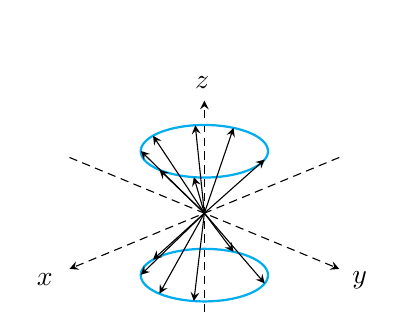
\begin{tikzpicture}
            \begin{axis}[
                view={-45}{-35},axis lines=center,densely dashed,
                xmax=3,xmin=-3,ymax=3,ymin=-3,zmax=5,zmin=-5,
                xtick=\empty,ytick=\empty,ztick=\empty
                ]

                \addplot3+[
                    thick,solid,cyan,
                    domain=0:2*pi,
                    samples=400, samples y=0,mark=none,
                ] ({sin(deg(x))},{cos(deg(x))},{2.75});
                \draw[-stealth,solid] (axis cs:0,0,0) -- (axis cs:{sin(deg(0))},{cos(deg(0))},2.75);
                \draw[-stealth,solid] (axis cs:0,0,0) -- (axis cs:{sin(deg(30))},{cos(deg(30))},2.75);
                \draw[-stealth,solid] (axis cs:0,0,0) -- (axis cs:{sin(deg(60))},{cos(deg(60))},2.75);
                \draw[-stealth,solid] (axis cs:0,0,0) -- (axis cs:{sin(deg(90))},{cos(deg(90))},2.75);
                \draw[-stealth,solid] (axis cs:0,0,0) -- (axis cs:{sin(deg(120))},{cos(deg(120))},2.75);
                \draw[-stealth,solid] (axis cs:0,0,0) -- (axis cs:{sin(deg(150))},{cos(deg(150))},2.75);
                \draw[-stealth,solid] (axis cs:0,0,0) -- (axis cs:{sin(deg(180))},{cos(deg(180))},2.75);

                \addplot3+[
                    thick,solid,cyan,
                    domain=0:2*pi,
                    samples=400,samples y=0,mark=none,
                ] ({sin(deg(x))},{cos(deg(x))},{-2.75});
                \draw[-stealth,solid] (axis cs:0,0,0) -- (axis cs:{sin(deg(0))},{cos(deg(0))},-2.75);
                \draw[-stealth,solid] (axis cs:0,0,0) -- (axis cs:{sin(deg(30))},{cos(deg(30))},-2.75);
                \draw[-stealth,solid] (axis cs:0,0,0) -- (axis cs:{sin(deg(60))},{cos(deg(60))},-2.75);
                \draw[-stealth,solid] (axis cs:0,0,0) -- (axis cs:{sin(deg(90))},{cos(deg(90))},-2.75);
                \draw[-stealth,solid] (axis cs:0,0,0) -- (axis cs:{sin(deg(120))},{cos(deg(120))},-2.75);
                \draw[-stealth,solid] (axis cs:0,0,0) -- (axis cs:{sin(deg(150))},{cos(deg(150))},-2.75);
            \end{axis}
        \node at (1.4,2){$x$};
        \node at (5.4,2){$y$};
        \node at (3.4,4.5){$z$};
        \end{tikzpicture} 
        }
        \begin{tikzpicture}
            \node at (0,0){};
            \draw[-stealth,solid] (0,1.5) -- node[above]{$\sum$} (1,1.5);
        \end{tikzpicture}
        \resizebox{0.44\linewidth}{!}{
        \begin{tikzpicture}
            \begin{axis}[
                view={-45}{-35},axis lines=center,densely dashed,
                xmax=3,xmin=-3,ymax=3,ymin=-3,zmax=5,zmin=-5,
                xtick=\empty,ytick=\empty,ztick=\empty
                ]

                \addplot3+[
                    thick,solid,white,
                    domain=0:2*pi,
                    samples=400, samples y=0,mark=none,
                ] ({sin(deg(x))},{cos(deg(x))},{2.75});

                \addplot3+[
                    thick,solid,white,
                    domain=0:2*pi,
                    samples=400,samples y=0,mark=none,
                ] ({sin(deg(x))},{cos(deg(x))},{-2.75});
            \draw[-stealth,solid,thick,red] (axis cs:0,0,0) -- (axis cs:0,0,3) node[right]{$M$};
            \end{axis}
        \node at (1.4,2){$x$};
        \node at (5.4,2){$y$};
        \node at (3.4,4.5){$z$};
        \end{tikzpicture} 
        }
        \caption{Omdannelse fra magnetiske momenter til bulk magnetisering ved summation. Antal molekyler i højt-- og lavt energistadie repræsenterer ikke virkeligheden.}
    \end{figure}

    Molekylet der undersøges vil have en række mulige energiniveauer givet ved:
    \[
        n_{\text{energistadier}}=2I+1
    \]
    Dette er hvad der gør analyse af molekyler med $I=\frac{1}{2}$ (eksempelvis $^1$H, $^{13}$C) specielt fordelagtigt, da det skaber et simpelt tilfælde med 2 mulige energistadier. Stadiernes energi, samt differensen mellem dem kan i det tilfælde beskrives ved:
    \[
        E_{\text{lav}}=-\frac{1}{2}h\gamma B_0 \hskip 32pt \Delta E=h\gamma B_0 \hskip 32pt E_{\text{høj}}=\frac{1}{2}h\gamma B_0
    \]
    Hvor $h$ er Plancks konstant. Det er denne energidifferens der muliggør analysen af molekylerne, da vi ved at udsætte dem for elektromagnetisk stråling med energi svarende til energidifferensen kan forårsage et \textit{spin flip}. Dvs.\ en overgang fra det lave energistadie til det høje. 
    \begin{figure}[H]
        \resizebox{\textwidth}{!}{
            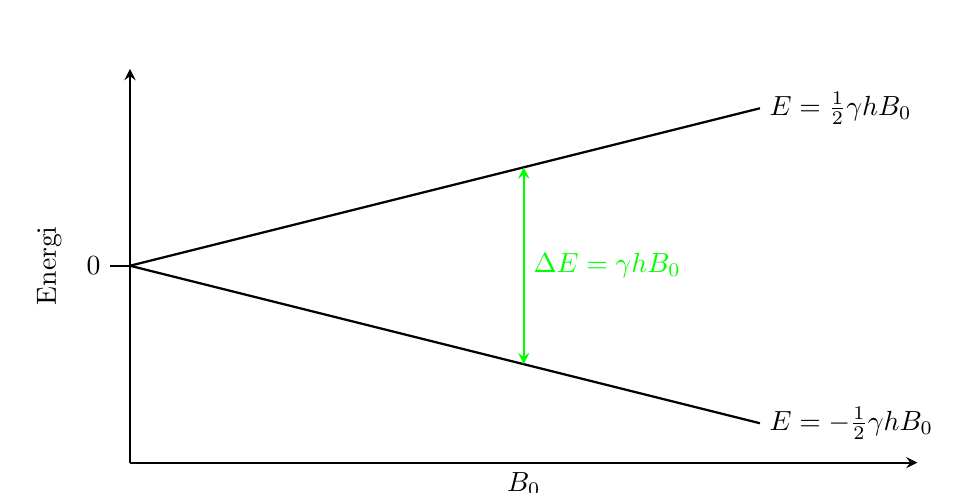
\begin{tikzpicture}
                \draw[-stealth,thick] (0,0) -- (0,5);
                \draw (-0.75,2.5) node [black,above,rotate=90] {Energi};
                \draw[-,thick] (0,2.5) -- (-0.25,2.5);
                \draw (-0.25,2.5) node [black,left] {$0$};
                \draw[-stealth,thick] (0,0) -- (10,0);
                \draw (5,0) node [black,below] {$B_0$};
                \draw[-,thick] (0,2.5) -- (8,4.5);
                \draw (8,4.5) node [black,right] {$E=\frac{1}{2}\gamma h B_0$};
                \draw[-,thick] (0,2.5) -- (8,0.5);
                \draw (8,0.5) node [black,right] {$E=-\frac{1}{2}\gamma h B_0$};
                \draw[stealth-stealth,green,thick] (5,1.25) -- (5, 3.75);
                \draw (5,2.5) node [green,right] {$\Delta E=\gamma h B_0$};
            \end{tikzpicture}
        }
        \caption{Stigning i energidifferens som funktion af magnetfeltets styrke.}
    \end{figure}
    Jf.\ Einstein-Planck relationen ved vi at energien af en foton er givet ved:
    \[
        E=hf
    \]
    og da denne skal være lig energidifferens må:
    \[
        \Delta E=hf \Leftrightarrow h\gamma B_0 =hf \Leftrightarrow \omega=\gamma B_0 
    \]
    Denne frekvens kaldes \textit{Larmor frekvensen}, noteret ved $\omega$, og angiver hyppigheden af bulk magnetiseringens præcession \parencite{Derr1,Derr2}.

    Det er præcis denne præcession der kan måles under analyse, da præcessionen af de ladede atomkerner inducerer en strøm, der kan måles i en spole viklet omkring prøvebeholderen. For at forårsage denne præcession indsendes radiofrekvente bølger, hvis frekvens er omkring $\omega$, i prøven sådan at $B_1 \perp B_0$. 

    Dette medfører at vores bulk magnetiseringsvektor ``tippes'' ud af ækvilibrium, ved at ændre atomernes spin og derved vende deres enkelte magnetiske momenter. Afhængigt af hvor længe prøven udsættes for dette ydre magnetfelt for, desto mere tipper magnetiseringsvektoren, vinklen er givet ved:
    \[
        \theta = \frac{\gamma B_1 \tau \cdot 180}{\pi}
    \]
    Hvor $\tau$ er tiden prøven udsættes for $B_1$ og $\gamma$ er det gyromagnetiske forhold.
        \begin{figure}[H]
        \resizebox{\linewidth}{!}{
        \begin{tikzpicture}
            \draw[-stealth,thick,densely dashed] (0,0) -- (4,0) node[right]{$x$}; 
            \draw[-stealth,thick,densely dashed] (0,0) -- (0,4) node[above]{$z$}; 
            \draw[-stealth,thick,densely dashed] (0,0) -- (-2,-3) node[below left]{$y$};
            \draw[-stealth,ultra thick,red] (0,0) -- +(90:3) node[right,red]{$M$};
            \draw[-stealth,ultra thick] (0,-3) -- (0,-1) node[right]{$B_0$};

            \draw[-stealth,thick,densely dashed] (8,0) -- (11,0) node[right]{$x$}; 
            \draw[-stealth,thick,densely dashed] (8,0) -- (8,4) node[above]{$z$}; 
            \draw[-stealth,thick,densely dashed] (8,0) -- (6,-3) node[below left]{$y$};
            \draw[-stealth,ultra thick,red] (8,0) -- +(45:2) node[right]{$M$};
            \draw[stealth-stealth,thick,cyan] (8,0.75) to[bend left] node[pos=.25,above right,font=\footnotesize]{$\qty{45}\degree$} (8.4,0.43);
            \draw[-stealth,ultra thick] (8,-3) -- (8,-1) node[right]{$B_0$};
            \draw[-stealth,ultra thick] (14,0) -- (12,0) node[below]{$B_1$};

            \draw[-stealth,thick,densely dashed] (18,0) -- (22,0) node[right]{$x$}; 
            \draw[-stealth,thick,densely dashed] (18,0) -- (18,4) node[above]{$z$}; 
            \draw[-stealth,thick,densely dashed] (18,0) -- (16,-3) node[below left]{$y$};
            \draw[stealth-stealth,thick,cyan] (18,0.75) to[bend left=45,font=\footnotesize] node[pos=.5,above right]{$\qty{90}\degree$} (18.75,0);
            \draw[-stealth,ultra thick,red] (18,0) -- +(0:3) node[below]{$M$};
            \draw[-stealth,ultra thick] (18,-3) -- (18,-1) node[right]{$B_0$};
            \draw[-stealth,ultra thick] (25,0) -- (23,0) node[below]{$B_1$};
            \node at (2,-4){(a)};
            \node at (11,-4){(b)};
            \node at (21.5,-4){(c)};
        \end{tikzpicture}
        }
        \caption{(a) Magnetiseringsvektoren i afslappet position, ingen ydre påvirkning. (b) Magnetiseringsvektoren bøjet $45\degree$ grundet ydre påvirkning fra $B_1$. (c) Magnetiseringsvektoren bøjet $90\degree$ grundet ydre påvirkning fra $B_1$.}
    \end{figure}
    Når den kortvarige puls ophører vil den begynde at præcessere omkring $B_0$. I denne forbindelse defineres 2 tidsintervaller:
    \begin{itemize}
        \item[$t_1$:] \textit{Spin-lattice relaxation time}, tiden det tager for bulk magnetiseringsvektoren at bevæge sig tilbage til startpositionen.
        \item[$t_2$:] \textit{Spin-spin relaxation time}, tiden det tager for $xy$-komponenterne af bulkmagnetiseringsvektoren igen at blive 0. 
    \end{itemize}
    Generelt vil $t_1 \geq t_2$, dette er dog ikke en regel, og nedenstående vil derfor ikke altid være sandt, da spin-lattice relaxation tiden ikke altid vil være den begrænsende faktor.
    \[
        \overrightarrow{M}=
        \begin{bmatrix}
            0 \\
            0 \\
            z
        \end{bmatrix}
        \stackrel{B_1}{\longrightarrow}
        \overrightarrow{M}=
        \begin{bmatrix}
            x \\
            y \\
            0
        \end{bmatrix}
        \stackrel{t_1}{\longrightarrow}
        \overrightarrow{M}=
        \begin{bmatrix}
            0 \\
            0 \\
            z
        \end{bmatrix}
    \]
    I takt med at magnetiseringsvektoren stabiliserer sig selv ved at præcessere, induceres en strøm grundet den spirallignende bevægelse i $xy$-planen, da det svarer til en ladning der bevæger sig.     
    \begin{figure}[H]
        \resizebox{\linewidth}{!}{
            \resizebox{0.62\linewidth}{!}{
            \begin{tikzpicture}
                \draw[-stealth,thick,densely dashed] (0,0) -- (4,0) node[right]{$y$}; 
                \draw[-stealth,thick,densely dashed] (0,0) -- (0,4) node[above]{$z$}; 
                \draw[-stealth,thick,densely dashed] (0,0) -- (-2,-3) node[below left]{$x$};
                \draw[stealth-stealth,thick,cyan] (0,0.75) to[bend left=45,font=\footnotesize] node[pos=.5,above right]{$\qty{90}\degree$} (0.75,0);
                \draw[-stealth,ultra thick,red] (0,0) -- (3,0) node[below]{M};
                \draw[-stealth,ultra thick] (0,-3) -- (0,-1) node[right]{$B_0$};
                \draw[-stealth,ultra thick] (7,0) -- (5,0) node[below]{$B_1$};
                \draw[-stealth,thick] (8,0) -- node[pos=.5,anchor=south]{$t_1$} (10,0);
            \end{tikzpicture}
            }
            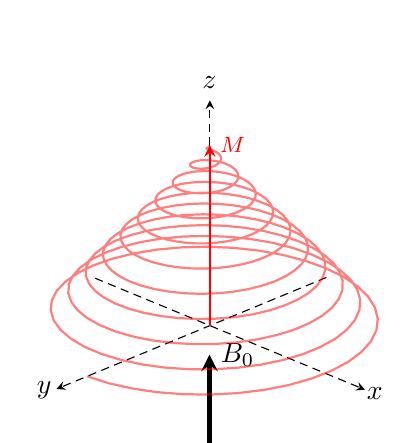
\begin{tikzpicture}
                \draw[-stealth,ultra thick] (3.4,0) -- (3.4,1.25) node[right]{$B_0$};
                \begin{axis}[
                    view={-45}{-35},
                    axis lines=center,
                    densely dashed,
                    xmax=2.5*pi,
                    ymax=2.5*pi,
                    zmax=2.5*pi,
                    xtick=\empty,
                    ytick=\empty,
                    ztick=\empty
                ]

                \addplot3+[
                    thick,
                    solid,
                    domain=0:2*pi,
                    samples=400,
                    samples y=0,
                    mark=none,
                    opacity=.5,
                    red,
                ] ({(2*pi-x)*sin(10*deg(x))},{(2*pi-x)*cos(10*deg(x))},{x});
                \draw[-stealth,thick,red,solid] (axis cs:0,0,0) -- (axis cs:0,0,2*pi) node[right,font=\footnotesize]{$M$};
            \end{axis}

            \node at (5.5,0.75){$x$};
            \node at (1.3,0.8){$y$};
            \node at (3.4,4.7){$z$};
        \end{tikzpicture}
        }
        \caption{Illustration af afslappelse fra exciteret tilstand ved præcession.}
    \end{figure}
    Grafen der dannes med udgangspunkt i den inducerede strøm kaldes \textit{FID}  (free induction decay), og giver os et eksponentielt faldende oscillerende signal, der ved Fourier transformation kan flyttes fra tidsdomænet, til frekvensdomænet \parencite{Davi2022}.
    \begin{figure}[H]
        \includegraphics[width=\textwidth]{billeder/fourier}
        \caption{Eksempler på omdannelser fra FID-grafer til NMR-spektra.}
    \end{figure}
    Hvor det vil være muligt at separere forskellige kemisk ækvivalente grupperinger af protoner, da deres Larmor frekvenser (og derved kemisk skift) vil være forskellige grundet gensidig beskyttelse fra det lokale elektronmiljø.

    \subsubsection{Kemisk skift}
    Toppene der ses i et H-NMR-spektrum må altså afhænge af Larmor-frekvensen for en given del af molekylet som der er bundet hydrogen til. Dette angives i kemisk skift, $\delta$, som er en værdi der opnås ved at samligne Larmor-frekvensen for delen af molekylet med en standard defineret af IUPAC, nemlig at $\delta_{\text{tetramethylsilan}}=0\si{ppm}$ \parencite{Robi2009}, hvilket muliggør beregning af kemisk skift ved:
    \[
        \delta = \frac{\omega_{\text{prøve}}-\omega_{\text{TMS}}}{\omega_{\text{TMS}}}
    \]
    Hvis enhed er \textit{ppm} (parts--per--million) da $\omega_{\text{TMS}}$ normalt angives i MHz og  $\omega_{\text{prøve}}$ i Hz. I nyere tid er det dog også blevet normalt at benytte opløsningsmidlets kemiske skift som en standard, og det noteres derfor altid med spektret. Umiddelbart lader det dog til at dette ville medføre at alle protonerne ville have ækvivalente kemiske skift, dette er dog ikke tilfældet, da de alle påvirkes af det ydre magnetiske felt forskellige grundet beskyttelse mod det grundet elektronerne der befinder sig omkring protonerne, eftersom elektroner per definition har et spin $I=\frac{1}{2}$, hvorved de danner et modsatrettet magnetfelt der skaber intereferens.

    For at identificere protoner der vil have forskellige grader af beskyttelse grundet deres lokale elektrondensitet undersøges de \textit{kemiske miljøer} der er tilstede i molekylet, dvs: ``hvilke protoner vil have den samme mængde beskyttelse mod det ydre magnetfelt''? Dette afhænger af molekylets symmetri. Et simpelt eksempel herpå et alkener:
    \begin{figure}[H]\centering
        \resizebox{0.5\textwidth}{!}{
            \chemfig{C(-[3]H)(-[5]H)=C(-[1]H)(-[7]H)}
        }
        \caption{Ethenmolekyle.}
    \end{figure}
    De 4 protoner i dette molekyle er kemisk ækvivalente, og de vil derfor have den samme Larmorfrekvens. Jf.\ symmetrien begrundes det i at molekylet i sig selv er fuldstændigt symmetrisk, samtidigt er det også klart at hver proton er bundet til et dobbeltbundet carbon. I større, mere komplekse molekyler kan de blive sværere at identificere kemisk ækvivalens. Se eksempelvis ethylparaben:
    \begin{figure}[H]\centering
        \resizebox{0.9\textwidth}{!}{
        \chemfig{\textcolor{green}{H}O-*6(=(-[5]\textcolor{blue}{H})-(-[7]\textcolor{red}{H})=(-C(-[7]O)(-[1]O(-C(-[2]\textcolor{cyan}{H})(-[6]\textcolor{cyan}{H})(-C(-[2]\textcolor{pink}{H})(-[6]\textcolor{pink}{H})(-\textcolor{pink}{H})))))-(-[1]\textcolor{red}{H})=(-[3]\textcolor{blue}{H})-)}
        }
        \caption{Ethylparaben med markerede kemisk ækvivalente protoner.}
    \end{figure}
    Her er der 5 adskilte kemiske miljøer i molekylet. Åbenlyst nok har protoner bundet på det samme carbon kemisk ækvivalens, forskellen i de kemiske miljøer for carbon--atomerne i alkylkæden begrundes hovedsageligt i afstanden til oxygen--atomet, grundet dets større elektronegativitet og derved indvirkning på elektrondensiteten omkring de nærliggende molekyler. I benzenringen er der to forskellige kemiske miljøer grundet dens symmetri, samt påvirkning af oxygen--atomet på phenolgruppen, samtidigt er det også klart at protonen vedhæftet oxygen--atomet må påvirkes meget kraftigt af oxygen--atomets elektronegativitet. 

    Naboprotoner har også mulighed for at skabe elektromagnetisk interfereres. Dette begrundes i at protonerne til enhver tid kan befinde sig i både det positive-- og negative spinstadie, hvorved de enten vil forstærke eller udligne det dannede magnetfelt. En generel regel kan derfor opstilles om at mængden af spidser der korresponderer til et givent kemisk miljø vil være givet ved $n+1$ hvor  $n$ er antallet af naboprotoner. For ethylparaben vil det sige at protonen på phenolgruppen vil have en enkelt spids, protonerne på benzenringen vil begge have 2, protonerne på methylengruppen vil have 4, mens dem på methylgruppen vil have 3 \parencite{Nana2020}.

    \subsubsection{IR--spektroskopi}
    Infrarød spektroskopi er en mindre selektiv spektroskopisk metode end H--NMR. Dog giver det stadig mulighed for identifikation af visse aspekter af et givent molekyle, hovedsageligt i form af funktionelle grupper.

    Ligesom i NMR--spektroskopi er det nødvendigt for molekylet man ønsker at undersøge at have et magnetisk moment. Dvs.\ at undersøgelse af symmetriske (H$_2$, N$_2$, O$_2$, osv.)-- samt monoatomige molekyler \textit{ikke} er muligt, da deres magnetiske momenter enten vil udligne hinanden eller ikke eksistere.

    Under IR--spektroskopi bestråles en prøve med infrarøde bølger. Hvis de præcist matcher enegidifferensen mellem molekylets grundstaide og exciterede stadie, sker der et spring i energistadie:
    \[
        \Delta E_{1 \rightarrow 2}
    \]
    hvilket får dem til at vibrere. Disse vibrationer manifesterers som en gentagen bevægelse af det kovalente bånd mellem atomerne, hvilket ligesom i NMR medfører en ændring i molekylets magnetiske moment der kan måles. Afhængigt af molekylstrukturen er der dog flere forskellige muligheder for vibrationer:
    \begin{table}[H]\center
        \caption{Mulige strækninger for molekyler af forskellige strukture.}
        \begin{tabular}{ccccc}
            \toprule
            & \multicolumn{2}{c}{Symmetrisk} & \multicolumn{2}{c}{Asymmetrisk} \\
            \cmidrule(r){2-3} \cmidrule(r){4-5}
            & Bøjning & Strækning & Bøjning & Strækning \\
            \midrule
            Monoatomig & $\times$ & $\times$ & $\times$ & $\times$ \\
            Diatomig & $\times$ & $\checkmark$ & $\times$ & $\times$ \\
            Triatomig & $\checkmark$ & $\checkmark$ & $\checkmark$ & $\checkmark$ \\
            Polyatomig & $\checkmark$ & $\checkmark$ & $\checkmark$ & $\checkmark$ \\
            \bottomrule
        \end{tabular}
    \end{table}
    I tilfældet med diatomige molekyler det simpelt at illustrere den mulige vibration da det kovalente bånd mellem dem udelukkende kan strækkes eller komprimeres, hvilket medfører en fjeder--lignende vibration.
    \begin{figure}[H]\centering
        \resizebox{0.75\linewidth}{!}{
            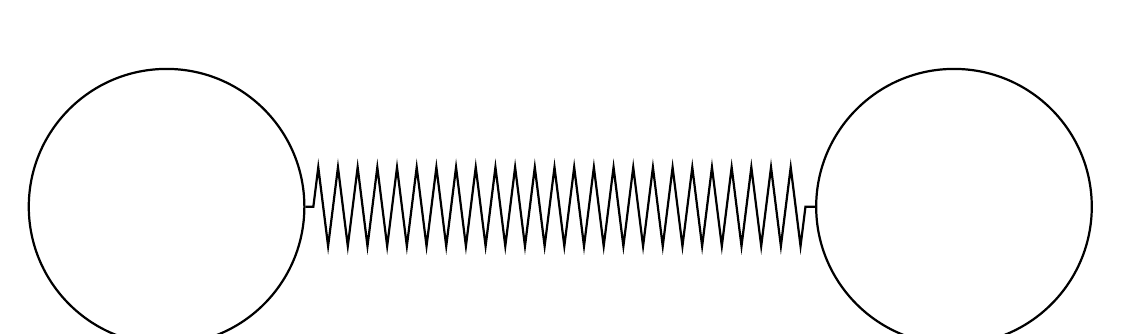
\begin{tikzpicture}
                \node[circle,draw,minimum size=3.5cm,thick] (A) at (0,0){};
                \node[circle,draw,minimum size=3.5cm,thick] (B) at (10,0){};
                \draw[thick,decoration={pre length=1mm, post length=1mm, segment length=2.5mm,amplitude=5mm,zigzag},decorate] (A) -- (B);
            \end{tikzpicture}
        }
        \caption{Kovalent bånd i diatomigt molekyle illustreret som fjeder.}
    \end{figure}
    For polyatomige molekyler bliver vibrationsmulighederne mere komplekse. Med udgangspunkt i triatomige molekyler kan mulighederne for de enkelte bånd dog illusteres. I takt med at flere atomer tilføjes kan vibrationerne dog kombineres på forskellige måder, samt påvirke hinanden, hvilket medfører en uendelig mængde mulige vibrationer.
    \begin{figure}[H]
        \resizebox{\linewidth}{!}{
            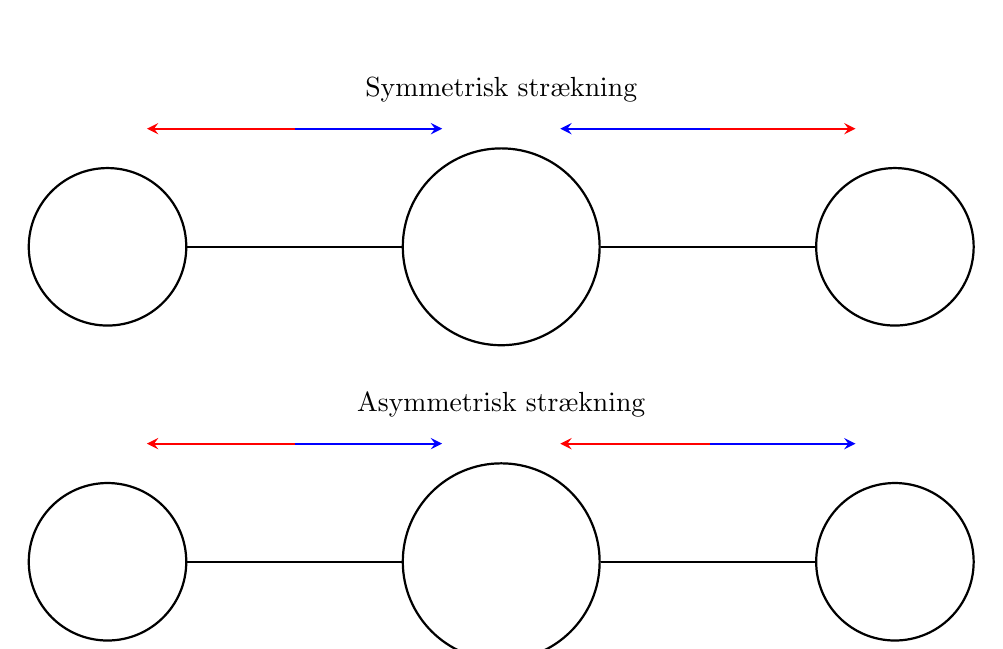
\begin{tikzpicture}
                \node[circle,draw,minimum size=2cm,thick] (A) at (0,0){};
                \node[circle,draw,minimum size=2.5cm,thick] (B) at (5,0){};
                \node at (5,2){Symmetrisk strækning};
                \node[circle,draw,minimum size=2cm,thick] (C) at (10,0){};
                \draw[-,thick] (A) -- (B);
                \draw[-,thick] (C) -- (B);
                \draw[-stealth,red,thick] (2.375,1.5) -- (0.5,1.5);
                \draw[-stealth,blue,thick] (2.375,1.5) -- (4.25,1.5);
                \draw[-stealth,red,thick] (7.65,1.5) -- (9.5,1.5);
                \draw[-stealth,blue,thick] (7.65,1.5) -- (5.75,1.5);
                
                \node[circle,draw,minimum size=2cm,thick] (D) at (0,-4){};
                \node[circle,draw,minimum size=2.5cm,thick] (E) at (5,-4){};
                \node at (5,-2){Asymmetrisk strækning};
                \node[circle,draw,minimum size=2cm,thick] (F) at (10,-4){};
                \draw[-,thick] (D) -- (E);
                \draw[-,thick] (F) -- (E);
                \draw[-stealth,red,thick] (2.375,-2.5) -- (0.5,-2.5);
                \draw[-stealth,blue,thick] (2.375,-2.5) -- (4.25,-2.5);
                \draw[-stealth,blue,thick] (7.65,-2.5) -- (9.5,-2.5);
                \draw[-stealth,red,thick] (7.65,-2.5) -- (5.75,-2.5);
            \end{tikzpicture}
        }
        \caption{Symmetrisk-- og asymmetrisk strækning af kovalente bånd i triatomigt molekyle.}
    \end{figure}
    
    \begin{figure}[H]
        \resizebox{\linewidth}{!}{
            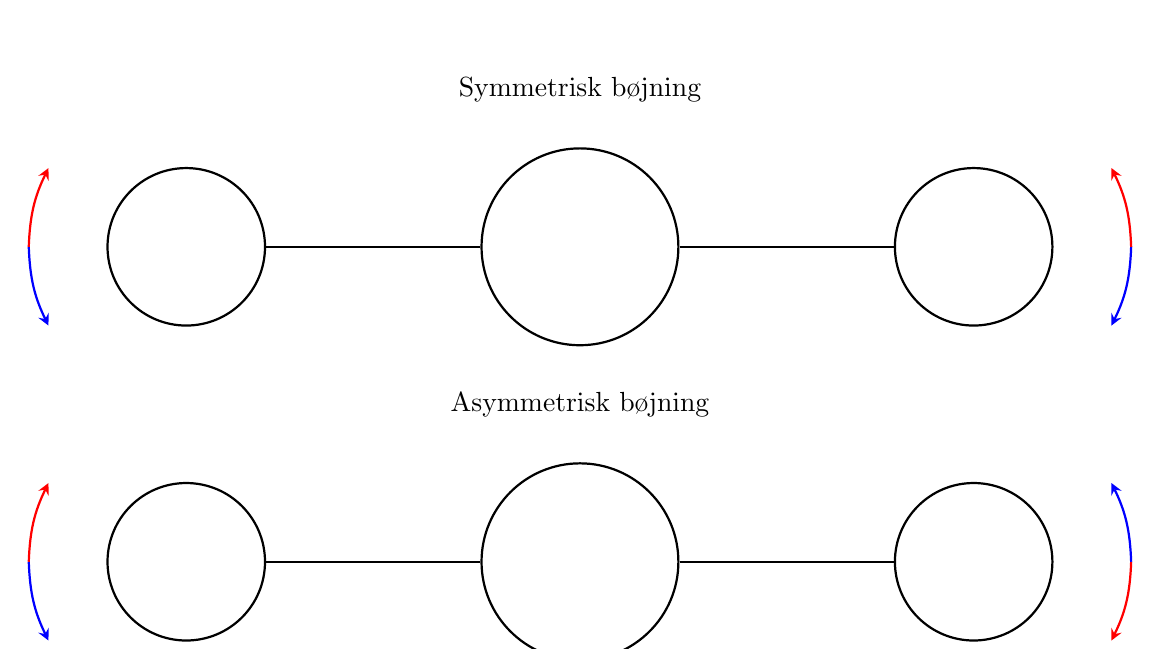
\begin{tikzpicture}
                \node[circle,draw,minimum size=2cm,thick] (a) at (0,0){};
                \node[circle,draw,minimum size=2.5cm,thick] (b) at (5,0){};
                \node at (5,2){Symmetrisk bøjning};
                \node[circle,draw,minimum size=2cm,thick] (c) at (10,0){};
                \draw[-,thick] (a) -- (b);
                \draw[-,thick] (c) -- (b);
                \draw[-stealth,blue,thick] (-2,0) to[bend right=12] (-1.75,-1);
                \draw[-stealth,red,thick] (-2,0) to[bend left=12] (-1.75,1);
                \draw[-stealth,blue,thick] (12,0) to[bend left=12] (11.75,-1);
                \draw[-stealth,red,thick] (12,0) to[bend right=12] (11.75,1);
                
                \node[circle,draw,minimum size=2cm,thick] (d) at (0,-4){};
                \node[circle,draw,minimum size=2.5cm,thick] (e) at (5,-4){};
                \node at (5,-2){Asymmetrisk bøjning};
                \node[circle,draw,minimum size=2cm,thick] (f) at (10,-4){};
                \draw[-,thick] (d) -- (e);
                \draw[-,thick] (f) -- (e);
                \draw[-stealth,blue,thick] (-2,-4) to[bend right=12] (-1.75,-5);
                \draw[-stealth,red,thick] (-2,-4) to[bend left=12] (-1.75,-3);
                \draw[-stealth,red,thick] (12,-4) to[bend left=12] (11.75,-5);
                \draw[-stealth,blue,thick] (12,-4) to[bend right=12] (11.75,-3);
            \end{tikzpicture}
        }
        \caption{Symmetrisk-- og asymmetrisk bøjning af kovalente bånd i triatomigt molekyle.}
    \end{figure}
    Bøjninger kan ske både i eget plan og vinkelret derpå hvis molekylet er lineært (eksempelvis CO$_2$). Dvs.\ at nogle molekyler ikke udelukkende har mulighed for at bøje fra side til side, men også frem og tilbage. Derudover bevæger det centrale molekyle sig også, da molekylets massemidtpunkt \textit{ikke} kan forskydes af vibrationerne.

    Mængden af mulige vibrationer er afhængigt af hvor mange frihedsgrader molekylet har. Idet atomer bevæger sig i et 3--dimensionelt rum, må hvert atom have 3 frihedsgrader, altså vil et molekyle have $3n$, hvor $n$ er mængden af atomer i molekylet, frihedsgrader.

    For udelukkende at undersøge de intermolekylære vibrationer fratrækkes de translatoriske-- og rotoriske frihedsgrader, og vi får derfor at det for ikke--lineære molekyler må være $3n-6$ frihedsgrader, og for lineære molekyler $3n-5$.

    Kigger vi eksempelvis på et diatomigt molekyle som HCl bliver det har klart at molekylet er lineært, samt at $n=2$. Der må altså være $3\cdot 2-5=1$ mulig vibration, hvilket stemmer, da den eneste mulige vibration er den fjederlignende bevægelse i det kovalente bånd.
    \begin{figure}[H]\centering
        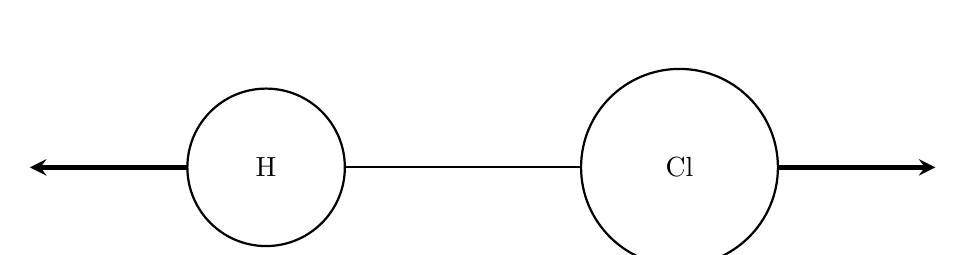
\begin{tikzpicture}
            \draw[thick] (0,0) circle (1) node{H} (5.25,0) circle (1.25) node{Cl};
            \draw[thick] (1,0) -- (4,0);
            \draw[-stealth,ultra thick] (-1,0) -- (-3,0); 
            \draw[-stealth,ultra thick] (6.5,0) -- (8.5,0);
        \end{tikzpicture}
        \caption{Frihedsgrader for lineært diatomigt molekyle.}
    \end{figure}
    For et ikke-lineært triatomigt molekyle, eksempelvis H$_2$O, vil vi i stedet hve $3\cdot 3-6=3$ frihedsgrader, der korresponderer til hhv.\ den symmetriske-- og asymmetriske strækning af de kovalente bånd, samt bøjning af bindingen til hydrogenatomerne \parencite{Theo2012}.
    \begin{figure}[H]
        \resizebox{\linewidth}{!}{
        \begin{tikzpicture}    
            \node[draw,circle,thick,minimum size=2cm] (a) at (0,0){H}; 
            \node[draw,circle,thick,minimum size=2.5cm] (b) at (3,.75){O}; 
            \node[draw,circle,thick,minimum size=2cm] (c) at (6,0){H};

            \node[draw,circle,thick,minimum size=2cm] (d) at (11,0){H}; 
            \node[draw,circle,thick,minimum size=2.5cm] (e) at (14,.75){O}; 
            \node[draw,circle,thick,minimum size=2cm] (f) at (17,0){H};

            \node[draw,circle,thick,minimum size=2cm] (g) at (5.5,-4.75){H};
            \node[draw,circle,thick,minimum size=2.5cm] (h) at (8.5,-4){O}; 
            \node[draw,circle,thick,minimum size=2cm] (i) at (11.5,-4.75){H};

            \draw[thick] (a) -- (b) (b) -- (c);
            \draw[thick] (d) -- (e) (e) -- (f);
            \draw[thick] (g) -- (h) (h) -- (i);

            \draw[-stealth,ultra thick] (a) -- (-2,-.5);
            \draw[-stealth,ultra thick] (c) -- (8,-.5);
            \draw[-stealth,ultra thick] (b) -- ++(0,2);

            \draw[-stealth,ultra thick] (d) -- (9,-.5); 
            \draw[stealth-,ultra thick] (f) -- (19,-.5);
            \draw[-stealth,ultra thick] (e) -- ++(2,0);

            \draw[-stealth,ultra thick] (g) -- ++(0,2); 
            \draw[-stealth,ultra thick] (i) -- ++(0,2);
            \draw[-stealth,ultra thick] (h) -- ++(0,-2);
        \end{tikzpicture}
        }
        \caption{Frihedsgrader for H$_2$O molekyle.}
    \end{figure}
    Indenfor IR--spektroskopi indføres et nyt mål for bølgelængden, \textit{bølgenummeret}, givet ved:
    \[
        \nu=\lambda^{-1}
    \]
    Med udgangspunkt i disse opdeles IR--området i 3 forskellige ``zoner'' \parencite{Shah2018}:
    \begin{itemize}
        \item[1)] NIR, $\nu \in \left[14000-4000\si{cm^{-1}}\right]$
        \item[2)] MIR, $\nu \in \left[4000-400\si{cm^{-1}}\right]$
        \item[3)] FIR, $\nu \in \left[400-40\si{cm^{-1}}\right]$
    \end{itemize}
    Til overordnet analyse benyttes ofte blot MIR--intervallet, da det er her man vil kunnet identificere de fleste funktionelle grupper og typer af bindinger, mens at FIR er langt mere komplekst og indeholder en stor mængde af vibrationer, hvilket gør det svært at type på. NIR korresponderer oftest til kombinationsvibrationer, eller ``molekylære overtoner'', spring i flere energistadier af gangen (eksempelvis $\Delta E_{1\rightarrow 3}$), hvilket igen gør det enormt svært at tyde dem.


    

    \section{Metoder}
    \subsection{Syntese} 
    Med udgangspunkt i den fundne syntesevejledning \parencite{Ole2019} udføres syntesen for ethyl-- og propylparaben grundet deres respektive alkoholers lavere farlighed end methanol. 

    Af samme grund benyttes ethanol som opløsningsmiddel under oprensningen, idet der herved helt undgås eksponering for methanol hvilket drastisk minimerer eksponeringen for farlige kemikalier under syntesen.

    Det vælges at producere 2 parabener for at muliggøre samligning af deres respektive H--NMR-- og IR--spektre, og begrunde hvorfor disse er opstået, samt at benytte dem i forbindelse med kvalitativ analyse til at vurdere det dannede produkts renhed. 

    Derudover giver det også mening jf.\ et eventuelt hæmningsforsøg at fravælge methylparaben da den generelt ses som havende en lavere effektivitet grundet dens ringere evne til at reagere med mikroorganismernes cellemembraner pga.\ større polaritet.

    Et flowdiagram for syntesen udarbejdes for at give overblik over syntesen, samt for at give bedre overblik gennem processen. Flowdiagrammet kan ses under bilag.

    Ca.\ 5g 4-hydroxybenzoesyre afvejes i rundbundet kolbe med slib:
    \begin{figure}[H] \centering
        \includegraphics[width=\textwidth]{billeder/afvejning}
        \caption{Afvejning af 4-hydroxybenzoesyre.}
    \end{figure} 
    Da syntesen sker med et overskud af alkohol vil der ideelt ske en fuldstændig reaktion. På baggrund heraf bestemmes det teoretiske udbytte ved at sætte dets stofmængde lig stofmængden af 4-hydroxybenzoesyre:
    \[
        n_{\text{4-hydroxybenzoesyre}}=\frac{5.1338\si{g}}{138.12\si{g \per mol}}=0.037169\si{mol}=n_{\text{ethylparaben}}
    \]
    Den teoretiske stofmængde af dannet ethylparaben omregnes nu til en masse hvorved det fås at:
    \[
        m_{\text{ethylparaben}}=0.037169\si{mol} \cdot 166.17\si{g\per mol}=6.1745g
    \]
    Et regneark udarbejdes til bestemmelsen af det teoretiske udbytte gennem de resterende synteser, en version med værdierne for denne syntese kan ses i bilag 2.

    Der afmåles nu 30mL ethanol i måleglas, hvorefter det overføres til den rundbundede kolbe. Kolben rystes til 4-hydroxybenzoesyren er fuldstændigt opløst, hvorefter 2.5mL svovlsyre tilsættes dråbevist under konstant forsigtig omrystning. 

    Opløsningen placeres i en varmekappe og forsynes med et svalerør for at koge med reflux i ca. 1 time for at forhindre fordampningen af alkoholen.
    \begin{figure}[H]
        \includegraphics[width=\textwidth]{billeder/opstilling}
        \caption{Forsøgsopstilling til syntesen.}
    \end{figure}
    Efter timen er gået slukkes varmekappen, hvorefter opløsningen nedkøles indtil det ikke længere er kogende og overføres til et 250mL bægerglas med 75mL demineraliseret vand. Bægerglasset placeres nu på en kogeplade og tilsættes en magnetomrører, hvorefter der sørges for moderat omrøring. Blandingen bestående af 10\% natriumcarbonat tilsættes nu opløsningen indtil udviklingen af gas stopper, hvorved svovlsyren vil være neutraliseret.

    Idet det ikke indgår i forsøgsvejledningen, udregnes mængden af natriumcarbonat der vil være nødvendig for at neutralisere svovlsyren, dog vil der under processen gøres brug af natriumcarbonat i overskud da det ingen negativ virkning vil have, eftersom temperaturen vil være for lav til at forsæbning af parabenen vil kunnet ske.

    Da svovlsyre har mulighed for at afgive 2 hydroner hvorved det reduceres til dets syrerest-ion, $\mathrm{SO_4^{2-}}$, må den tilsatte base kunnet optage 2 hydroner for at netrualisere 1 svovlsyremolekyle:
    \begin{figure}[H]
        \resizebox{\textwidth}{!}{
        \schemestart
        \chemfig{S(=[1]O)(=[3]O)(-[5]OH)(-[7]OH)}
        \+
        \chemfig{H_{2}O}
        \arrow{->}
        \chemfig{S(=[1]O)(=[3]O)(-[5]OH)(-[7]O^{-})}
        \+
        \chemfig{H^{+}}
        \arrow{->}
        \chemfig{S(=[1]O)(=[3]O)(-[5]O^{-})(-[7]O^{-})}
        \+ 2
        \chemfig{H^{+}}
        \schemestop
        }
        \caption{Dissociering af svovlsyre ved tilsættelse til vand.}
    \end{figure}
    Samtidig er det klart at natriumcarbonat har mulighed for at optage 2 hydroner da det ved tilsættelse til vand øjeblikkeligt dissocierer til natrium-- og carbonat--ioner, der herefter reagerer videre for at danne natriumhydroxid.
    \begin{figure}[H]
        \resizebox{\textwidth}{!}{
        \schemestart
        \chemfig{C(=[2]O)(-[5]NaO)(-[7]ONa)}
        \+
        \chemfig{H_{2}O}
        \arrow{->}
        \chemfig{C(-[3]O^{-})(-[5]O^{-})=O}
        \+ 2
        \chemfig{Na^{+}}
        \schemestop
        }
        \caption{Dissociering af natriumcarbonat ved tilsættelse til vand.}
    \end{figure}
    Carbonat--ionen har mulighed for at reagere med vand hvorved der dannes bicarbonat og en hydroxid--ion, bicarbonat--ionen reagerer videre med vand for at danne ustabil kulsyre og endnu en hydroxidion, hvorefter den ustabile kulsyre brydes hvilket medfører dannelsen af carbondioxid og vand. 
    \begin{align}
        \mathrm{CO_3^{2-} + H_2O} &\longrightarrow \mathrm{HCO_3^- + OH^-} \\
        \mathrm{HCO_3^- + H_2O} &\longrightarrow \mathrm{H_2CO_3 + OH^-} \\
        \mathrm{H_2CO_3} &\longrightarrow \mathrm{CO_2 + H_2O}
    \end{align}
    De dannede hydroxidioner har nu mulighed for at reagere med hydronerne dannet af svovlsyren, mens natriumionerne har mulighed for at reagere med sulfationerne.
    \begin{align*}
        \mathrm{OH^- + H^}+ &\longrightarrow \mathrm{H_2O} \\
        \mathrm{2Na^+ + SO_4^{2-}} &\longrightarrow \mathrm{Na_2SO_4}
    \end{align*}
    Dette muliggør opskrivning som en totalreaktion ved:
    \begin{figure}[H]
        \resizebox{\textwidth}{!}{
        \schemestart
        \chemfig{C(=[2]O)(-[5]NaO)(-[7]ONa)}
        \+
        \chemfig{S(=[1]O)(=[3]O)(-[5]OH)(-[7]OH)}
        \arrow{->}
        \chemfig{S(-ONa)(-[4]NaO)(=[2]O)(=[6]O)}
        \+
        \chemfig{C(=O)(=[4]O)}
        \+ 2
        \chemfig{H_{2}O}
        \schemestop
        }
        \caption{Totalreaktion mellem svovlsyre og natriumcarbonat i vandig opløsning.}
    \end{figure}
    Da det nu er klart at reaktionen mellem svovlsyre og natriumcarbonat foregår i forholdet 1:1 og at der under syntesen benyttes 2.5mL svovlsyre med en densitet på $1.84\si{g \per mL}$ må det være nødvendigt at bruge:
    \[
        n_{\text{svovlsyre}}=\frac{2.5\si{mL} \cdot 1.84\si{g\per mL}}{98.08\si{g\per mol}}=0.04690mol
    \]
    natriumcarbonat til at neutralisere svovlsyren. Stofmængden omregnes til en masse af natriumcarbonat, her er det vigtigt at pointere at der benyttes natriumcarbonatdecahydrat under fremstillingen af opløsningen, grundet dets effekt på molvægten.
    \[
        m_{\text{natriumcarbonat}}=0.04690\si{mol} \cdot 286.14\si{g\per mol}=13.4200\si{g}
    \]
    Da det ikke skaber et problem at tilsætte natriumcarbonat i overskud laves opløsning ved brug af 15g natriumcarbonatdecahydrat og $150\si{mL}$ vand. En 10\% opløsning benyttes for at reducere voldsomheden af reaktionen mellem den stærke syre og base, samt for at modvirke dens store eksotermicitet.

    Den neutraliserede opløsning sugefiltreres og skylles 3 gange med demineraliseret vand efter afkøling. Det isolerede krystallinske stof overføres til et $250\si{mL}$ bægerglas. Samtidigt opvarmes $50\si{mL}$ hhv.\ ethanol og vand til opvarmning i hvert deres bægerglas. Når ethanolen koger opløses det krystallinske stof i så lidt som muligt hvorefter varmt vand tilsættes til opløsningen bliver uklar.

    Opløsningen stilles nu til frivillig nedkøling, hvorved parabenen igen udfældes og kan isoleres ved sugefiltrering i afvejet glasfilterdigel. Det dannede produkt stilles til tørring i glasfilterdiglen benyttet til filtreringen, hvorefter udbyttet bestemmes ved afvejning.

    \subsection{Smeltepunktsbestemmelse}
    Smeltepunktsbestemmelsen udføres først med udgangspunkt i et kommercielt indkøbt produkt for at have et teoretisk smeltepunkt hvilket gør det muligt at på forhånd undgå systematiske afvigelser. 

    En smule af de kommercielt købte produkter stampes op i et lukket kapillærrør, hvorefter det ``droppes'' gentagne gange for at komprimere produktet. Det placeres nu i smeltepunktsbestemmelsesapparetet, som varmes op til en temperatur $10\si{\degree C}$ lavere end det forventede smeltepunkt, hvorefter vi langsomt varmer op indtil produktet smelter.
    \begin{figure}[H]\centering
        \caption{Teoretisk smeltepunkt for ethyl-- og propylparaben.}
        \begin{tabular}{ccc}
            \toprule
            & \multicolumn{2}{c}{Smeltepunkt $\left[\si{\degree C}\right]$} \\
            \cmidrule(r){2-3}
            Prøve # & Ethylparaben & Propylparaben \\
            \midrule
            1 & 117 & 97 \\
            2 & 115 & 94 \\
            3 & 117 & 95 \\
            \midrule
            Gennemsnit & 116.3 & 95.3 \\
            \bottomrule
        \end{tabular}
    \end{figure}
    Disse værdier benyttes fremadrettet som gældende tabelværdier. Prøven udføres nu på samme måde med produkterne fremstillet ved syntese for at muliggøre sammenligning af deres smeltepunkt.

    \subsection{TLC--analyse}
    Produkt dannet ved syntese samt dets kommercielle modstykke opløses i ethanol for at muliggøre påsætning på TLC--plade. Til dette formål benyttes en løbevæske bestående af $80\%$ heptan og $20\%$ ethylacetat (polaritetsindeks hhv.\ 0.0 og 4.4 \parencite{Phen}), da andre lod til at have success med dette forhold.

    En streg tegnes ca.\ $1\si{cm}$ over TLC--pladens bund, og prøvemateriale påsættes pladerne med et åbent kapillærrør, hvorefter de placeres i et bægerglas med et lille lag løbevæske i bunden, og dækkes med et urglas.

    Når løbevæskefronten når ca. $1\si{cm}$ fra toppen af TLC--pladen udtages de, og lægges til tørring til løbevæsken er fordampet, hvorefter de bestråles med UV--lys og stofplaceringerne markeres.

    \subsection{NMR--spektroskopi}
    Prøven sendes til Aarhus Universitet som udfører analysen.

    \subsection{IR--spektroskopi}
    Prøven sendes til Aarhus Universitet som udfører analysen.

    \subsection{Hæmningsforsøg}
    Et hæmningsforsøg udføres også for at undersøge parabenernes hæmmende vækst på forskellige bakterier. Med udgangspunkt i litteraturen er det klart at parabener er mere effektive mod Gram--positive end Gram--negative bakterier \parencite{Joao2021}, grundet den øgede beskyttelse fra den ydre polypeptide cellemembran. 

    Derudover har tidligere studier undersøgt de effektive koncentrationer for væksthæmning ved de forskellige parabener for bakteriearterne \parencite{Wies2019}. Grundet dette undersøges 2 forskellige bakterier, \textit{bacilius cereus} og \textit{escherichia coli}, for at muliggøre undersøgelse af både et gram--positivt og gram--negativt bakterie:
    \begin{table}[H]\centering
        \caption{Karakteristika, MIC og navn på udvalgte baktierier.}
        \begin{tabular}{cccc}
            \toprule
            & & \multicolumn{2}{c}{MIC $\left[\si{W\per W\%}\right]$} \\
            \cmidrule(r){3-4}
            Bakterieart & Cellevægsstruktur & Ethylparaben & Propylparaben \\
            \midrule
            \textit{bacillus cereus} & Gram--positiv & 0.1 & 0.0125 \\
            \textit{escherichia coli} & Gram--negativ & 0.1--0.125 & 0.05--0.1 \\
            \bottomrule
        \end{tabular}
    \end{table}
    
    \subsubsection{Agar--diffusion}
    I laboratorier benyttes agar--diffusion til at afprøve og sammenligne forskellige antibiotikas effekt på en isoleret bakteriekultur. Dette gøres ved at opløse antibiotikaet i et passende opløsningsmiddel som papirdiske derefter vædes i, hvorefter de stilles til tørring. Disse spredes over en Muller--Hinton--agarplade podet med bakteriearten man ønsker at undersøge, og stilles så til inkubering. 

    Antibiotikaet der befinder sig i papirdisken vil \textit{diffundere}, dvs.\ vandre fra papirdisken og ud i agaren, hvilket medfører ad der vil være en radius omkring disken hvor der ingen vækst er (hvis det antibakterielle middel er effektivt).
    \begin{figure}[H]\centering
        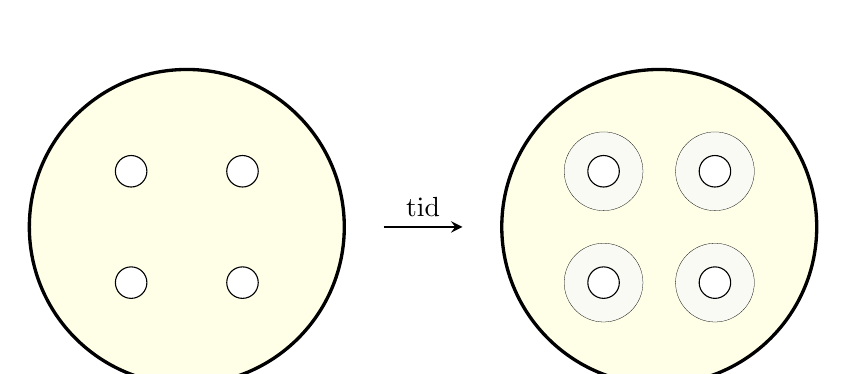
\begin{tikzpicture}
            \filldraw[very thick,fill=yellow!10] (0,0) node(a){} circle (2);
            \filldraw[very thick,fill=yellow!10] (6,0) node(b){} circle (2);

            \draw[-stealth,thick] (2.5,0) -- node[above]{tid} (3.5,0);

            \foreach \x in {45,135,-45,-135}
                \filldraw[fill=gray!5, fill opacity=.75,ultra thin] (b)+(\x:1) circle (0.5);

            \foreach \x in {a,b}
                \foreach \y in {45,135,-45,-135}
                \filldraw[fill=white] (\x)+(\y:1) circle (0.2);
        \end{tikzpicture}
        \caption{Diffusion af stof indeholdt i papirdiske.}
    \end{figure}
    Den vækstfrie radius vil afhænge af antibiotikaens effektivitet, da koncentrationen vil falde i takt med at stoffet diffunderer længere og længere ud. Med udgangspunkt heri kan et kvalitativt gæt på den minimum inhibitoriske koncentration opstilles.
    \begin{figure}[H]\centering
        \begin{tikzpicture}
            \filldraw[very thick,fill=yellow!10] (0,0) node(a){} circle (2);


            \draw[-stealth,thick] (2.5,0) -- node[above]{vækst} (3.5,0);

            \filldraw[very thick,fill=yellow!10] (6,0) node(b){} circle (2);

            \filldraw[pattern={Lines[angle=45,distance=1.5mm]},pattern color=black] (6,0) circle (1.99);

            \filldraw[fill=yellow!10,very thin] (b)+(45:1) circle (0.3);
            \filldraw[fill=yellow!10,very thin] (b)+(135:1) circle (0.75);
            \filldraw[fill=yellow!10,very thin] (b)+(-135:1) circle (0);
            \filldraw[fill=yellow!10,very thin] (b)+(-45:1) circle (0.5);

            \foreach \x in {a,b}
                \foreach \y in {45,135,-45,-135}
                \filldraw[fill=white] (\x)+(\y:1) circle (0.2);

            \node[font=\footnotesize] at (.71,.71) {$c$};
            \node[font=\footnotesize] at (.71,-.71) {$d$};
            \node[font=\footnotesize] at (-.71,.71) {$a$};
            \node[font=\footnotesize] at (-.71,-.71) {$b$};

            \node[font=\footnotesize] at (6.71,.71) {$c$};
            \node[font=\footnotesize] at (6.71,-.71) {$d$};
            \node[font=\footnotesize] at (5.29,.71) {$a$};
            \node[font=\footnotesize] at (5.29,-.71) {$b$};

        \end{tikzpicture}
        \caption{Illustration af hæmningsradius. MIC: $b>c>d>a$.}
    \end{figure}
    Det samme princip benyttes her med parabenerne. En mættet parabenopløsning bestående af ethanol og paraben fremstilles hvorefter de sterile papirdiske vædes deri, de stilles herefter til tørring for at minimere ethanolens egen bakteriehæmmende virkning.

    Papirdiskene placeres på en poddet Mueller--Hinton--agarplade, hvorefter de let præsses ned på agarpladen med en flamme--steriliseret pincet for at sikre overfladekontakt. Pladerne stilles herefter til inkubering natten over, hvorefter radius af de hæmmende zoner måles.
    \begin{figure}[H]\centering
        \includegraphics[width=.75\linewidth]{billeder/mhplade}
        \caption{Poddet Muller--Hinton--agarplade med parabenvæddede papirdiske.}
    \end{figure}

    \subsubsection{Fortyndingsrække}
    Modsat agar--diffusion benyttes fortyndingsrækker til at bestemme definitive værdier (eller værdi--intervaller) af den minimale inhibitoriske koncentration for forskellige antibakterielle midler (antibiotika, konserveringsmidler, osv.). 

    Dette gøres ved at opstille en fortyndingsrække i et bakteriefyldt medie med det antibaktierelle stof man ønsker at undersøge. Ved at have forskellige koncentrationer af stoffet, og herefter følge udviklingen i OD600 over tid, kan man undersøge hvordan de forskellige koncentrationer påvirker bakterievæksten.
    \begin{figure}[H]\centering
        \begin{tikzpicture}[scale=.97]
            \fill[blue!99.9] (-3,.5) rectangle ++(1,-.5) (-3,0) to[bend right=90,looseness=1.25] (-2,0) (-2.5,.5) ellipse (.5 and .2);
            \fill[blue!88.8] (0,0) rectangle ++(0.4,0.5) (0,0) to[bend right=90, looseness=1.75] ++(0.4,0);
            \fill[blue!77.7] (1.25,0) rectangle ++(0.4,0.5) (1.25,0) to[bend right=90, looseness=1.75] ++(0.4,0);
            \fill[blue!66.6] (2.5,0) rectangle ++(0.4,0.5) (2.5,0) to[bend right=90, looseness=1.75] ++(0.4,0);
            \fill[blue!55.5] (3.75,0) rectangle ++(0.4,0.5) (3.75,0) to[bend right=90, looseness=1.75] ++(0.4,0);
            \fill[blue!44.4] (5,0) rectangle ++(0.4,0.5) (5,0) to[bend right=90, looseness=1.75] ++(0.4,0);
            \fill[blue!33.3] (6.25,0) rectangle ++(0.4,0.5) (6.25,0) to[bend right=90, looseness=1.75] ++(0.4,0);
            \fill[blue!22.2] (7.5,0) rectangle ++(0.4,0.5) (7.5,0) to[bend right=90, looseness=1.75] ++(0.4,0);
            \fill[blue!11.1] (8.75,0) rectangle ++(0.4,0.5) (8.75,0) to[bend right=90, looseness=1.75] ++(0.4,0);
            
            \draw[-,thick] (-3,1.5) -- (-3,0) (-2,0) -- (-2,1.5) (-3,0) to[bend right=90,looseness=1.25] node[below]{Parabenopløsning} (-2,0) (-3,0) to[bend left=90,looseness=1.25,opacity=.5] (-2,0);
            \draw[thick] (-2.5,1.5) ellipse (0.5 and 0.25) node(a)[above]{};
            \draw[thick,opacity=.4] (-2.5,.5) ellipse (.5 and .2);
            \draw[-stealth,thick] (a) to[bend left=75,looseness=1.25] node[above,font=\footnotesize]{$100\si{\mu l}$} (0,2.25)

            \draw[-,densely dotted,thick] (-.5,.5) node[left,font=\footnotesize]{$100\si{\mu l}$} --  (9.65,.5);
            
            \foreach \x in {0,1.25,...,8.75}{
                \draw[thick] (\x,0) --  ++(0,2);
                \draw[thick] ($(\x+0.4,0)$) -- ++(0,2);
                \draw[-,thick] (\x,0) to[bend right=90,looseness=1.75] ++(0.4,0);
                \draw[thick] ($(\x+0.2,2)$) ellipse (.2 and .1);
            }

            \foreach \x in {0.4,1.65,...,8.25}
            \draw[-stealth,thick] (\x,2.25) to[bend left=90,looseness=1.25] node[above,font=\footnotesize]{$100\si{\mu l}$} ++(.85,0);
            }
        \end{tikzpicture}
        \caption{Fortynding ved gentagen overførsel fra brønd til brønd.}
    \end{figure}

    Fortynding som illustreret ovenfor medfører en halvering af koncentrationen fra brønd til brønd, beskrevet ved rekursionsligningen:
    \[
        c_n=c_{\text{opløsning}}\cdot 0.5^n, n \in \left\{1,2,3,...,n\right\}
    \]
    Vi opstiller nu en fortyndingsrække hvor den 7.\ brønd svarer til den højeste teoretiske MIC:
    \[
        1.25\si{mg\per mL}=c_{\text{opløsning}}\cdot 0.5^7 \Leftrightarrow c_{\text{opløsning}}=\frac{1.25\si{mg\per mL}}{0.5^7}=160\si{mg\per mL}
    \]
    Da det er nødvendigt at vente på at ethanolen fordamper, ønsker vi at nå den nødvendige koncentration med så lille en mængde ethanol som muligt. En mættet opløsning af ethylparaben i ethanol indeholder $550\si{mg\per mL}$, dvs.\ at det må være nødvendigt at overføre:
    \[
        160\si{mg}=550\si{mg\per mL} \cdot V_{\text{ethanol}} \Leftrightarrow V_{\text{ethanol}}=\frac{160\si{mg}}{550\si{mg\per mL}}=290\si{\mu L}
    \]
    Da vi arbejder med en brøndvolumen på $100\si{\mu L}$ benytter vi en 10.\ del af dette. En fortyndingsrække opstiles derfor ved at fylde brøndene med $29\si{\mu L}$ ren ethanol, hvorefter det fortyndes med den mættede opløsning.

    De samme beregninger udføres for propylparaben hvorved vi har at:
    \[
        160\si{mg}=746\si{mg\per mL} \cdot V_{\text{ethanol}} \Leftrightarrow V_{\text{ethanol}}=\frac{160\si{mg}}{746\si{mg\per mL}}=210\si{\mu L}
    \]
    Altså benyttes $21\si{\mu L}$ under opstillingen af propylfortyndingsrækken, hvilket vil resultere i koncentrationer givet ved:
    \begin{figure}[H]\centering
        \begin{tikzpicture}[scale=.76,every node/.style={scale=.76}]
            \fill[blue!100] (-3,.5) rectangle ++(1,-.5) (-3,0) to[bend right=90,looseness=1.25] (-2,0) (-2.5,.5) ellipse (.5 and .2);
            \fill[blue!92.3] (0,0) rectangle ++(0.4,0.5) (0,0) to[bend right=90, looseness=1.75] ++(0.4,0);
            \fill[blue!84.6] (1.25,0) rectangle ++(0.4,0.5) (1.25,0) to[bend right=90, looseness=1.75] ++(0.4,0);
            \fill[blue!76.9] (2.5,0) rectangle ++(0.4,0.5) (2.5,0) to[bend right=90, looseness=1.75] ++(0.4,0);
            \fill[blue!69.2] (3.75,0) rectangle ++(0.4,0.5) (3.75,0) to[bend right=90, looseness=1.75] ++(0.4,0);
            \fill[blue!61.5] (5,0) rectangle ++(0.4,0.5) (5,0) to[bend right=90, looseness=1.75] ++(0.4,0);
            \fill[blue!53.8] (6.25,0) rectangle ++(0.4,0.5) (6.25,0) to[bend right=90, looseness=1.75] ++(0.4,0);
            \fill[blue!46.2] (7.5,0) rectangle ++(0.4,0.5) (7.5,0) to[bend right=90, looseness=1.75] ++(0.4,0);
            \fill[blue!38.5] (8.75,0) rectangle ++(0.4,0.5) (8.75,0) to[bend right=90, looseness=1.75] ++(0.4,0);
            \fill[blue!30.8] (10,0) rectangle ++(0.4,0.5) (10,0) to[bend right=90, looseness=1.75] ++(0.4,0);
            \fill[blue!23.1] (11.25,0) rectangle ++(0.4,0.5) (11.255,0) to[bend right=90, looseness=1.75] ++(0.4,0);
            \fill[blue!15.4] (12.5,0) rectangle ++(0.4,0.5) (12.5,0) to[bend right=90, looseness=1.75] ++(0.4,0);
            \fill[blue!7.7] (13.75,0) rectangle ++(0.4,0.5) (13.75,0) to[bend right=90, looseness=1.75] ++(0.4,0);
            
            \draw[-,thick] (-3,1.5) -- (-3,0) (-2,0) -- (-2,1.5) (-3,0) to[bend right=90,looseness=1.25] node(a)[below,font=\footnotesize]{$160\si{mg\per mL}$} (-2,0) (-3,0) to[bend left=90,looseness=1.25,opacity=.5] (-2,0);
            \draw[thick] (-2.5,1.5) ellipse (0.5 and 0.25) node(a)[above]{};
            \draw[thick,opacity=.4] (-2.5,.5) ellipse (.5 and .2);
            \draw[-stealth,thick] (a) to[bend left=75,looseness=1.25] node[above,font=\footnotesize]{$100\si{\mu l}$} (0,2.25)

            \draw[-,densely dotted,thick] (-.5,.5) node[left,font=\footnotesize]{$100\si{\mu l}$} --  (14.65,.5);
            \draw[decorate,decoration={brace}] (14.25,-.75) -- node[below]{koncentration $\left[\si{mg\per mL}\right]$} (-.1,-.75);
            
            \foreach \x in {0,1.25,...,13.75}{
                \draw[thick] (\x,0) --  ++(0,2);
                \draw[thick] ($(\x+0.4,0)$) -- ++(0,2);
                \draw[-,thick] (\x,0) to[bend right=90,looseness=1.75] ++(0.4,0);
                \draw[thick] ($(\x+0.2,2)$) ellipse (.2 and .1);
            }

            \foreach \x in {0.4,1.65,...,13.25}
            \draw[-stealth,thick] (\x,2.25) to[bend left=90,looseness=1.25] node[above,font=\footnotesize]{$100\si{\mu l}$} ++(.85,0);
            }

            \draw[-stealth] (7.7,3.25) node[above,font=\footnotesize]{Teoretisk MIC} -- (7.7,2.25);

            \node[font=\scriptsize] at (0.2,-.45){$80$};
            \node[font=\scriptsize] at (1.45,-.45){$40$};
            \node[font=\scriptsize] at (2.7,-.45){$20$};
            \node[font=\scriptsize] at (3.95,-.45){$10$};
            \node[font=\scriptsize] at (5.2,-.45){$5$};
            \node[font=\scriptsize] at (6.45,-.45){$2.5$};
            \node[font=\scriptsize] at (7.7,-.45){$1.25$};
            \node[font=\scriptsize] at (8.95,-.45){$0.63$};
            \node[font=\scriptsize] at (10.2,-.45){$0.31$};
            \node[font=\scriptsize] at (11.45,-.45){$0.16$};
            \node[font=\scriptsize] at (12.7,-.45){$0.078$};
            \node[font=\scriptsize] at (13.95,-.45){$0.039$};
        \end{tikzpicture}
        \caption{Koncentrationer i ELISA--brønde afrundet til 2 decimaler.}
    \end{figure}
    Efter ethanolen i brøndene er fordampet er vi efterladt med de korresponderende mængder af paraben. Måling af MIC ved svært opløselige produkter kan være svært, da det i praksis medfører at vi vil have et lag uopløst paraben liggende i bunden af brønden. For parabener gør dette sig også gældende ved teoretisk MIC, da den befinder sig over begge parabeners opløselighed i vand. 

    Dog er der nogle faktorere der medfører at opløseligheden ``stiger'' i praksis. Bl.a. parabenernes evne til at reagere med de lipide bakteriecellemembraner, hvilket medfører en større opløselighed i mediet, samt at OD600--målingerne foregår ved højere temperatur (inkubationstemperatur, $30\si{\degree C}$) end stuetemperatur.

    $100\si{\mu L}$ en--dags inkuberet LB--medie poddet med bakterierne vi ønsker at undersøge fortyndes til $A_{600} \in \left[0.1;0.2\right]$ og overføres til hver brønd. En skematisk illustration af opstillingen kan ses nedenfor:
    \begin{figure}[H]\centering
        \resizebox{\linewidth}{!}{
        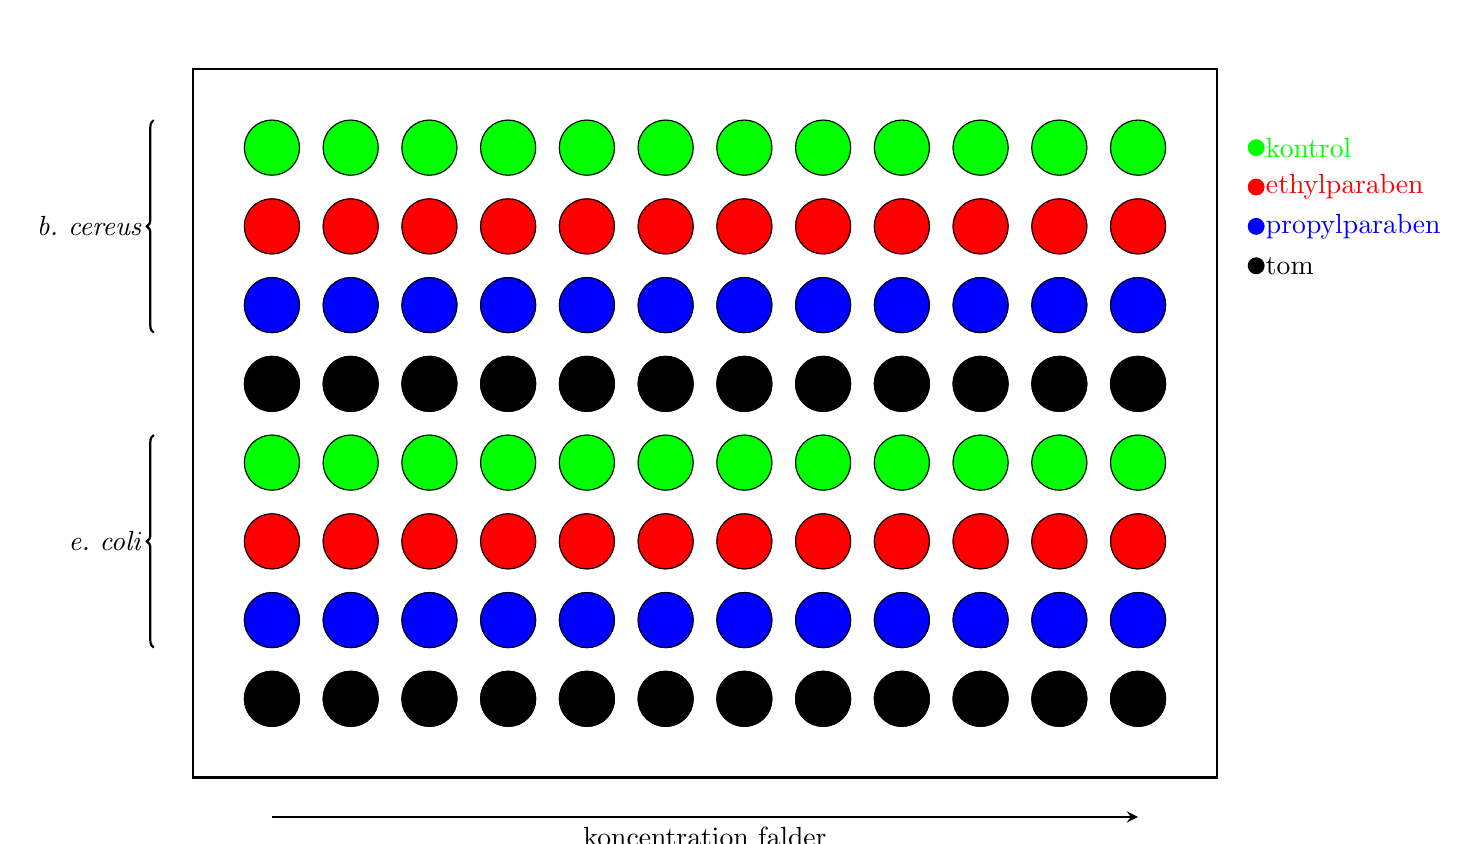
\begin{tikzpicture}
            \draw[thick] (0,0) rectangle (13,9);
            \foreach \x in {1,2,...,12}
                \foreach \y in {4,8}
                \filldraw[green] (\x,\y) circle (0.35);
            \foreach \x in {1,2,...,12}
                \foreach \y in {2,6}
                \filldraw[blue] (\x,\y) circle (0.35);
            \foreach \x in {1,2,...,12}
                \foreach \y in {3,7}
                \filldraw[red] (\x,\y) circle (0.35);
            \foreach \x in {1,2,...,12}
                \foreach \y in {1,5}
                \filldraw[black] (\x,\y) circle (0.35);
            \foreach \x in {1,2,...,12}
                \foreach \y in {1,2,...,8}
                    \draw (\x,\y) circle (0.35);
            \draw[decoration={brace},thick,decorate] (-.5,1.65) -- node[left]{\textit{e. coli}} (-.5,4.35);
            \draw[decoration={brace},thick,decorate] (-.5,5.65) -- node[left]{\textit{b. cereus}} (-.5,8.35);
            \filldraw[black] (13.5,6.5) circle (.1) node[right]{tom};
            \filldraw[blue] (13.5,7) circle (.1) node[right]{propylparaben};
            \filldraw[red] (13.5,7.5) circle (.1) node[right]{ethylparaben};
            \filldraw[green] (13.5,8) circle (.1) node[right]{kontrol};
            \draw[-stealth,thick] (1,-.5) -- node[below]{koncentration falder} (12,-.5);

        \end{tikzpicture}
        }
        \caption{Skematisk illustration af ELISA--opstilling.}
    \end{figure}
    Pladen placeres i ELISA--readeren hvorefter der udføres absorbtionsmålinger ved $595\si{nm}$ (ca.\ OD600) hver 15.\ minut over 20 timer. Dette gør det muligt for os at følge bakterievæksten, og derved undersøge hvilken indvirkning parabenerne har derpå. 

    Med udgangspunkt heri bestemmes hhv.\ MIC90, MIC50 og MIC10, der svarer til parabenkoncentrationerne der medfører en vækstreduktion på $90\%$, $50\%$ og  $10\%$, hvilket herefter sammenlignes med teoretiske værdier fra opslag i litteraturen.

    Umiddelbart har vi forventninger til nogle afvigende målinger i brøndene med højeste koncentrationer, da parabenen ikke kan holdes opløst og derfor vil ophobe sig på bunden af brøndene, hvilket vil gøre det nødvendigt at rydde op i de indsamlede data.
 
    
    \section{Resultatbehandling og diskussion}

    \subsection{Smeltepunkt og TLC}
    \begin{figure}[H]\centering
        \caption{Smeltepunkt og RF (retentionsfaktor) for stof dannet ved de 3 synteser, samt sammenligning med teoretiske værdier for kommercielt stof.}
        \begin{tabular*}{\linewidth}{c@{\extracolsep{\fill}}cccccccc}
            \toprule
            & & & & & \multicolumn{4}{c}{Syntese 3} \\
            \cmidrule(r){6-9}
            & \multicolumn{2}{c}{Syntese 1} & \multicolumn{2}{c}{Syntese 2} & \multicolumn{2}{c}{Ethyl} & \multicolumn{2}{c}{Propyl} \\
            \cmidrule(r){2-3} \cmidrule(r){4-5} \cmidrule(r){6-7} \cmidrule(r){8-9}
            Prøve \# & SMP & RF & SMP & RF & SMP & RF & SMP & RF \\
            \midrule
            1 & 116 & 0.24 & 95 & 0.63 & 116 & 0.50 & 96 & 0.49 \\
            2 & 115 & 0.20 & 96 & 0.67 & 116 & 0.49 & 93 & 0.45 \\
            3 & 116 & 0.21 & 96 & 0.59 & 117 & 0.49 & 94 & 0.45 \\
            \midrule
            Teoretisk & 117 & 0.22 & 97 & 0.63 & 117 & 0.49 & 97 & 0.46 \\
            Gennemsnit & 116 & 0.22 & 95.7 & 0.63 & 116.3 & 0.49 & 94.3 & 0.46 \\
            \midrule
            Afvigelse $\left[\si{\%}\right]$ & -1 & 0 & -1 & 2 & -1 & 0 & -3 & 0 \\
            \bottomrule
        \end{tabular*}
    \end{figure} \vskip -8pt
    Med udgangspunkt i hhv.\ smeltepunkts-- samt TLC--analysen vil det være rimeligt at antage at det dannede stof sandsynligvis er hvad vi tror det er. De relativt høje afvigelser for smeltepunktet hos propylparaben kan hovedsageligt tilskrives større partikelstørrelse, da pulveret var svært at knuse ordentligt hvilket medførte mindre tæt pakning.

    \subsection{H--NMR--spektroskopi}
    Vi undersøger først spektret for ethylparaben og vurderer om det er sandsynligt at det dannede H NMR-spektrum passer til det vi ville forvente. Til dette formål kigger vi på de individuelle peaks da antallet af spidser kan give os en ide om hvilke atomer de korresponderer til.
    \begin{figure}[H] \centering
        \includegraphics[width=\textwidth,page=2]{bilag/ethylnmr}
        \caption{Peaks for H--NMR analyse af ethylparaben.}
    \end{figure} 
    Peaket omkring $\delta=1.28\si{ppm}$ forventes at være tilsvarende methylgruppen på forgreningen der udgår fra benzenringen, eftersom vi observerer 3 peaks, må atomet hydrogenerne er bundet til have 2 naboprotoner, hvilket kun opfyldes af methylengruppen. Ved $\delta=4.25\si{ppm}$ ses 4 peaks, altså må det være methylengruppen idet den har 3 naboprotoner fra methylgruppen. 
    
    Omkring $\delta=6.84\si{ppm}$ forventer vi hydrogenerne bundet til carbonatomerne i meta-positionerne i benzenringen, idet de vil have et lavere kemisk skift end dem i ortho-positionen grundet den øgede elektronegativitet fra oxygenatomet der er til stede i phenolgruppen. 
    
    I selve spektret ses også en singlet ved $\delta=10.25\si{ppm}$, dette kemiske skift er højere end hvad vi normalt villet forvente for en phenolgruppe (der normalt villet befinde sig omkring det aromatiske område, ligesom ortho- og meta-carbonatomerne). Dette kan begrundes i det benyttede opløsningsmiddel, DMSO-d6, da det har mulighed for at danne hydrogenbindinger med phenolgruppen \parencite{Raym2007}
    \begin{figure}[H]\centering
        \resizebox{\textwidth}{!}{
        \schemestart
        \chemfig{HO-*6(=-=(-COOR)-=-)}
        \+
        \chemfig[-32pt]{S(-[7]CD3)(-[5]CD3)(=[2]O)}
        \arrow(.mid east--.mid west){->}
        \chemfig{O(=[5]S(-[3]CD3)(-[6]CD3))-[2,,,,thick,dotted,red]H(-[1]O-*6(=-=(-COOR)-=-))}
        \schemestop
        }
        \caption{Dannelse af hydrogenbinding mellem DMSO-d6 og vilkårlig paraben.}
    \end{figure}
    Dette medfører at deres elektronegativitet ``mødes i midten'', hvorved den lokale elektrondensitet på hydrogenatomet (og derved beskyttelsen mod $B_0$) øges drastisk.
    \begin{figure}[H] \centering
        \includegraphics[width=\textwidth,page=2]{bilag/propylnmr}
        \caption{Peaks for H--NMR analyse af propylparaben.}
    \end{figure} 

    \subsection{IR--spektroskopi}


    \subsection{Hæmningsforsøg}
    


    
    \include{diskussion.tex}

    \section{Konklusion}
Vores smeltepunkter for både det kommercielle-- og produktet fremstilt ved syntese afveg meget lidt fra hinanden, hvilket er indikativt for renhed grundet manglen på potentielle biprodukter. Derudover afveg vores TLC--analyser også meget lidt fra det for kommercielle produkt. 

Samtidigt viste de mere selektive spektroskopiske analyser også minimale afvigelser fra teoretiske-- og praktiske spektra, hvilket bekræfter vores mere kvantitative analysers i at det dannede produkt er det vi ønskede.

De hæmmende egenskaber af parabenerne var også som forventede. De bestemte MIC--værdier afveg relativt meget ved \textit{bacillus cereus}--mediet, dog passede de nærmest en--til--en med \textit{escherichia coli}--mediet.

Med udgangspunkt i undersøgelsen af de fysiske karakteristika--, spektroskopiske molekylinteraktioner samt den hæmmende effekt er det derfor sikkert at konkludere at det dannede produkt er hvad vi ønskede at danne ved syntesen, samt stor renhed.

    
    \pagebreak

    \printbibliography[heading=bibnumbered]

    \pagebreak

    \appendix

    \captionsetup{font={color=white}}

    \section{Flowchart}
    \begin{figure}[H] \centering
        \includegraphics[width=\textwidth]{bilag/flowdiagram}
        \caption{}
    \end{figure} 
    
    \section{Mængdeberegninger}
    \subsection{Ethylparaben}
    \begin{table}[H]\centering
        \resizebox{\textwidth}{!}{
        \begin{tabular}{ccccc}
            \toprule
            Stof & Mængde $\left[\si{g} \vee \si{mL}\right]$ & Densitet $\left[\si{g\per mL}\right]$ & MV $\left[\si{g\per mol}\right]$ & Stofmængde $\left[\si{mol}\right]$ \\
            \midrule
            4-hydroxybenzoesyre & 5.1338 & & 138.12 & 0.0372 \\
            Ethanol & 30 & 0.79 & 46.07 & 0.514 \\
            Teoretisk ethylparaben & 5.66 & & & \\
            Praktisk ethylparaben & 2.2666 & & & \\
            \midrule
            Afvigelse & -60\% \\
            \bottomrule
        \end{tabular}
        }
        \caption{} \vskip -32pt
    \end{table}

    \subsection{Propylparaben}
    \begin{table}[H]\centering
        \resizebox{\textwidth}{!}{
        \begin{tabular}{ccccc}
            \toprule
            Stof & Mængde $\left[\si{g} \vee \si{mL}\right]$ & Densitet $\left[\si{g\per mL}\right]$ & MV $\left[\si{g\per mol}\right]$ & Stofmængde $\left[\si{mol}\right]$ \\
            \midrule
            4-hydroxybenzoesyre & 5.0346 & & 138.12 & 0.0365 \\
            Propanol & 30 & 0.803 & 60.1 & 0.401 \\
            Teoretisk propylparaben & 5.55 & & & \\
            Praktisk propylparaben & 4.4144 & & & \\
            \midrule
            Afvigelse & -20\% \\
            \bottomrule
        \end{tabular}
        }
        \caption{} \vskip -24pt
    \end{table}


    \subsection{Dobbeltsyntese}
    \begin{table}[H]\centering
        \resizebox{\textwidth}{!}{
        \begin{tabular}{ccccc}
            \toprule
            Stof & Mængde $\left[\si{g} \vee \si{mL}\right]$ & Densitet $\left[\si{g\per mL}\right]$ & MV $\left[\si{g\per mol}\right]$ & Stofmængde $\left[\si{mol}\right]$ \\
            \midrule
            4-hydroxybenzoesyre & 5.0176 & & 138.12 & 0.0363 \\
            Ethanol & 30 & 0.79 & 46.07 & 0.514 \\
            Teoretisk ethylparaben & 5.53 & & & \\
            Praktisk ethylparaben & 2.4244 & & & \\
            \midrule
            Afvigelse & -56\% \\
            \bottomrule
        \end{tabular}
        }
        \caption{} \vskip -12pt
    \end{table}
    
    \begin{table}[H]\centering
        \resizebox{\textwidth}{!}{
        \begin{tabular}{ccccc}
            \toprule
            Stof & Mængde $\left[\si{g} \vee \si{mL}\right]$ & Densitet $\left[\si{g\per mL}\right]$ & MV $\left[\si{g\per mol}\right]$ & Stofmængde $\left[\si{mol}\right]$ \\
            \midrule
            4-hydroxybenzoesyre & 5.0346 & & 138.12 & 0.0365 \\
            Propanol & 30 & 0.803 & 60.1 & 0.401 \\
            Teoretisk propylparaben & 5.55 & & & \\
            Praktisk propylparaben & 0.5692 & & & \\
            \midrule
            Afvigelse & -90\% \\
            \bottomrule
        \end{tabular}
        }
        \caption{} \vskip -24pt
    \end{table}
    
    \captionsetup{font={color=black}}
    \section{TLC--plader}
    \subsection{Syntese 1}
    \begin{figure}[H]
        \includegraphics[width=0.48\linewidth]{billeder/tlc1}
        \includegraphics[width=0.48\linewidth]{billeder/tlcmarkeret1}
        \caption{TLC--plader fra syntese 1, eget produkt til venstre og kommercielt til højre}
    \end{figure} \vskip -24pt

    \subsection{Syntese 2}
    \begin{figure}[H]
        \includegraphics[width=0.48\linewidth]{billeder/tlc2}
        \includegraphics[width=0.48\linewidth]{billeder/tlcmarkeret2}
        \caption{TLC--plader fra syntese 2, eget produkt til venstre og kommercielt til højre}
    \end{figure} \vskip -24pt

    \subsection{Dobbeltsyntese}
    \begin{figure}[H]
        \includegraphics[width=0.48\linewidth]{billeder/tlc3}
        \includegraphics[width=0.48\linewidth]{billeder/tlcmarkeret3}
        \caption{TLC--plader fra syntese 3, første 2 er ethylparaben, næste 2 er propylparaben, eget produkt til venstre og kommercielt til højre}
    \end{figure} \vskip -24pt

    \captionsetup{font={color=white}}
    \addcontentsline{toc}{section}{H--NMR--Spektre}

    \includepdf[pages=-,landscape=true,addtotoc={1,subsection,2,Ethylparaben,ethylspek,2,subsubsection,3,Peaks,ethylpeaks}]{bilag/ethylnmr.pdf}

    \includepdf[pages=-,landscape=true,addtotoc={1,subsection,2,Propylparaben,propylspek,2,subsubsection,3,Peaks,propylpeaks}]{bilag/propylnmr.pdf}

    \addcontentsline{toc}{section}{IR--Spektre}

    \includepdf[pages=-,landscape=true,addtotoc={1,subsection,1,Ethylparaben,ethylir}]{bilag/ethylir.pdf}

    \includepdf[pages=-,landscape=true,addtotoc={1,subsection,1,Propylparaben,propylir}]{bilag/propylir.pdf}

    \includepdf[pages={1,2,3},addtotoc={1,section,1,Risikovurdering,risikovurdering}]{bilag/risikovurdering.pdf}


\end{document}
